% based on a template made by the university of cologne
% http://www.mi.uni-koeln.de/wp-MIEDV/wp-content/uploads/2016/07/LaTeX-Vorlage.zip - 2023-11-02
\documentclass[12pt,a4paper]{scrartcl}

\addtokomafont{sectioning}{\rmfamily}
\usepackage[ngerman]{babel}% deutsches Sprachpaket wird geladen
\usepackage[T1]{fontenc} % westeuropäische Codierung wird verlangt
\usepackage[utf8]{inputenc}% Umlaute werden erlaubt
\usepackage[usenames]{color} % Erlaubt die Benutzung der namen im Farbpaket und deren Änderung
\usepackage{amsmath} % Erweiterung für den Mathe-Satz
\usepackage{amssymb} % alle Zeichen aus msam und msmb werden dargestellt
\usepackage{graphicx} % Graphiken und Bilder können eingebunden werden
%\usepackage{multirow} % erlaubt in einer Spalte einer Tabelle die Felder in mehreren Zeilen zusammenzufassen
\usepackage{enumerate} % erlaubt Nummerierungen
\usepackage{xurl} % Dient zur Auszeichnung von URLs; setzt die Adresse in Schreibmaschinenschrift.
\usepackage[center]{caption}  % Bildunterschrift wird zentriert
%\usepackage{subfigure} % mehrere Bilder können in einer fugure-Umgebung verwendet werden
%\usepackage{longtable} % Diese Umgebung ist ähnlich definiert wie die tabular-Umgebung, erlaubt jedoch mehrseitige Tabellen.
%\usepackage{paralist} % Modifikation der bereits bestehenden Listenumgebungen
\usepackage{lmodern}% Für die Schrift
\usepackage[hidelinks]{hyperref} % Links und Verweise werden innerhalb von PDF Dokumenten erzeugt
%\usepackage{wrapfig} % Das Paket ermöglicht es von Schrift umflossene Bilder und Tabellen einzufügen.
\usepackage{latexsym} % LaTeX-Symbole werden geladen
\usepackage{tikz} % Erlaubt es mit tikz zu zeichnen
\usepackage{tabularx} % Erlaubt Tabellen
\usepackage{algorithm} % Erlaubt Pseudocode
\usepackage{color} % Farbpaket wird geladen
%\usepackage{stmaryrd} % St Mary Road Symbole werden geladen
\usepackage{physics}
\usepackage[version=4]{mhchem} % Chemie: \ce & \pu

\numberwithin{equation}{section} % Nummerierungen der Gleichungen, die durch equation erstellt werden, sind gebunden an die section
\newcommand{\code}[1]{\textsf{#1}}
\newcommand{\HRule}{\rule{\linewidth}{0.7mm}}
\newcommand{\pu}[1]{\ensuremath{\mathrm{#1}}}

\hyphenation{An-samm-lung }
\hyphenation{auf-wen-dig}
\hyphenation{Brems-me-di-ums}
\hyphenation{be-schreibt}
\hyphenation{Cu-rie-Tem-pe-ra-tur}
\hyphenation{Dop-pel-ätz-me-tho-de}
\hyphenation{ei-ner-seits}
\hyphenation{ein-ge-stellt}
\hyphenation{e-lek-tro-mag-ne-tische}
\hyphenation{Ener-gie-stragg-ling}
\hyphenation{Ent-mag-neti-sier-ungs-fak-tor}
\hyphenation{Ent-mag-neti-sier-ungs-feld-stär-ke}
\hyphenation{Ent-mag-neti-sier-ungs-ver-hal-ten}
\hyphenation{Erd-be-schleu-ni-gung}
\hyphenation{Er-eig-nis-se}
\hyphenation{er-kenn-bar}
\hyphenation{er-rei-chen}
\hyphenation{ge-ra-der}
\hyphenation{Ge-schoss-e-ner-gi-en}
\hyphenation{Ge-schwin-dig-keit}
\hyphenation{Grenz-be-reich}
\hyphenation{Koh-len-stoff-ket-ten}
\hyphenation{Kom-mu-tie-rungs-kur-ve}
\hyphenation{konn-te}
\hyphenation{kor-ri-gier-te}
\hyphenation{Li-te-ra-tur-wer-te}
\hyphenation{Li-thi-um-fluo-rid-Kris-tal-len}
\hyphenation{Mag-ne-ti-sier-ungs-aus-rich-tung}
\hyphenation{nach-ge-wie-sen}
\hyphenation{nächs-ten}
\hyphenation{nä-he-rungs-wei-se}
\hyphenation{Nor-mal-ver-tei-lung}
\hyphenation{or-ga-ni-schen}
\hyphenation{Pri-mär-elek-tron}
\hyphenation{Scha-len-mo-dells}
\hyphenation{Schnitt-flä-che}
\hyphenation{Se-kun-där-elek-tron-en}
\hyphenation{Se-kun-där-elek-tron-en-ver-viel-fach-er}
\hyphenation{statt-fin-det}
\hyphenation{sys-te-ma-tisch-en}
\hyphenation{Ver-ar-mungs-zo-ne}
\hyphenation{vi-su-a-li-siert}
\hyphenation{Wie-der-ho-lung}
\hyphenation{zu-sätz-lich}


\hypersetup{
  pdftitle={B1.1},
  pdfcreator={LaTeX via pandoc}}

\setcounter{secnumdepth}{6}
\setcounter{tocdepth}{6}

\begin{document}
\begin{titlepage}
	\pagestyle{empty}

	\begin{center}

	\textsc{\LARGE Universität zu Köln }\\ [0.4cm]
	\textsc{Mathematisch-Naturwissenschaftliche Fakultät} \\[1.5cm]

	
\includegraphics[width=0.45\textwidth]{../media/uni.jpg}\\[1.5cm]  % Uni-Logo wird geladen

	\textsc{\Large Praktikum~B}\\[2mm]
	\textsc{}\\[10mm]
	\HRule \\[0.4cm]

		{	\Huge \bfseries B1.1}\\[0.4cm]
			{	\huge \bfseries Infrarotabsorption in $\ce{CO_2}$}\\[0.3cm]
	
	\HRule \\[3cm]

 	\begin{center}
		\textsc{\Large Catherine~Tran } \\[3pt]
		\textsc{\Large Carlo~Kleefisch } \\[3pt]
		\textsc{\Large Oliver~Filla } \\[3pt]
	\end{center}
	\end{center}
\end{titlepage}

\newpage
\tableofcontents
\newpage

\hypertarget{einleitung}{%
\section{Einleitung}\label{einleitung}}

Mithilfe von Spektroskopie ist es möglich, Absorptions- und Emissionsspektren von elektromagnetischen Wellen an einer Probe zu beobachten. Hierzu misst man spezifische Größen in Abhängigkeit von der Frequenz. Dadurch ist es möglich, Aussagen über die mikroskopischen Eigenschaften der Probe zu treffen.

Alternativ zur Frequenz werden auch äquivalente Größen wie der Wellenlänge oder Energie verwendet, um Größen wie die Intensität, die Strahlungsleistung und die Zählrate der Strahlung zu messen.

Dieser Versuch dient als Einführung in die Infrarotspektroskopie. Mithilfe eines niedrig auflösenden Absorptionsspektrometers wird die Infrarot--Absorption von Kohlenstoffdioxid $(\ce{CO_2})$ untersucht. Dieses Gas gehört zu den sogenannten ``Treibhausgasen''.

\clearpage
\hypertarget{theoretische-grundlagen}{%
\section{Theoretische Grundlagen}\label{theoretische-grundlagen}}

\hypertarget{treibhauseffekt}{\subsection{Treibhauseffekt}\label{treibhauseffekt}}
Die Temperatur auf der Photosphäre der Sonne beträgt ca. $6000\mathrm{\,K}$ \cite{BakanRaschke}. Von der Erde aus lässt sich diese Größe ungefähr über das Stefan--Boltzmann--Strahlungsgesetz \eqref{eq:SBS} berechnen, wozu die Stefan-Boltzmann Konstante $\sigma$ und die Oberfläche $A$ der Sonne benötigt werden. \cite{Gerthsen}

\begin{eqnarray}
	P &=& \sigma \cdot A \cdot T_\mathrm{eff}^{\,4} \label{eq:SBS} \\
	\sigma &=& 5.67 \cdot 10^{-8} \mathrm{\,\frac{W}{m^2K^4}}
\end{eqnarray}

\noindent
Eine andere Möglichkeit der Temperaturbestimmung nutzt das Wien'sche Verschiebungsgesetz \eqref{eq:Wien Verschiebungsgesetz}. Das Emissionsspektrum der Sonne hat ein Maximum bei $\hat \nu=3.4 \cdot 10^{14} \mathrm{\,Hz}$, woraus sich die Temperatur $T$ ermitteln lässt. \cite{Gerthsen}

\begin{eqnarray}
	\hat \nu &=& 5.88 \cdot10^{10} \cdot T \label{eq:Wien Verschiebungsgesetz}
\end{eqnarray}

\noindent
Das solare Maximum des Spektrums liegt bei einer Wellenlänge von $0.6\mathrm{\,\mu m}$ und ist in Abbildung \ref{abb:Spektrum Sonne & Erde} oben dargestellt. Das Sonnenlicht wird von Stoffen in der Atmosphäre und Erdoberfläche stark absorbiert. Bei irdischen Temperaturen emittieren unserer Erdboden und Atmosphäre wieder Strahlungen im Infrarotbereich ab, dadurch wird die Erde aufgewärmt und das Leben ermöglicht. \cite{BakanRaschke}

Die Erdatmosphäre besteht aus $78.1\,\%$ Stickstoff $\ce{N_2}$, $20.9\,\%$ Sauerstoff $\ce{O_2}$, $0.93\,\%$ Argon $\ce{Ar}$, $1.45\,\%$ Wasserdampf $\ce{H_2O}$ und $1\,\%$ aus sogenannen Treibhausgasen. Zu den Treibhausgasen zählen Kohlenstoffdioxid $\ce{CO_2}$, Methan $\ce{CH_4}$, Distickstoffmonoxid $\ce{N_2O}$ und Ozon $\ce{O_3}$.

Dabei tragen Wasserdampf und die Treibhausgase am meisten zu dem atmosphärischen Treibhauseffekt bei. Ohne sie wäre unsere Erdoberfläche im Durchschnitt um $33\mathrm{\,^\circ C}$ kälter. \cite{BakanRaschke}

Kohlenstoffdioxid und Wasserdampf prägen das Absorptionspektrum stark, was in Abbildung \ref{abb:Spektrum Sonne & Erde} ebenfalls dargestellt ist. Was absorbiert wurde, wird nach dem kirchhoff'schen Strahlungsgesetz auch wieder emittiert.

Bei einer Wellenlänge unter $0.5\mathrm{\,\mu m}$ erfolgt die Energieabsorption durch atomare Übergänge, liegen die Wellenlänge allerdings höher dann passiert es durch Übergänge zwischen Rotations- und Schwingungszuständen. Dies ist auch der Grund, warum Stoffe wie Sauerstoff und Stickstoff im Infrarotbereich nicht absorbieren, sie besitzen kein Dipolmoment und können auch keines durch Rotation oder Schwingungen bekommen. \cite{BakanRaschke}

Neben dem natürlichen Treibhauseffekt gibt es noch einen anthropogenen Treibhauseffekt, der sich negativ auf das Klimasystem auswirkt. In den letzten $150$ Jahren hat sich der Anteil der Treibhausgase durch wirtschaftliche, landschaftliche und soziale Entwicklungen erheblich erhöht, sodass mehr Sonnenstrahlungen absorbiert und somit auch mehr Wärmestrahlungen abgegeben werden. In Erdbodennähe steigt die Temperatur, während in der Strato- und Mesosphäre eine Abkühlung stattfindet. Dies führt schließlich zu einer Destabilisierung der gesamten Atmosphäre. \cite{BakanRaschke}

\begin{figure}[h!]
	\centering
	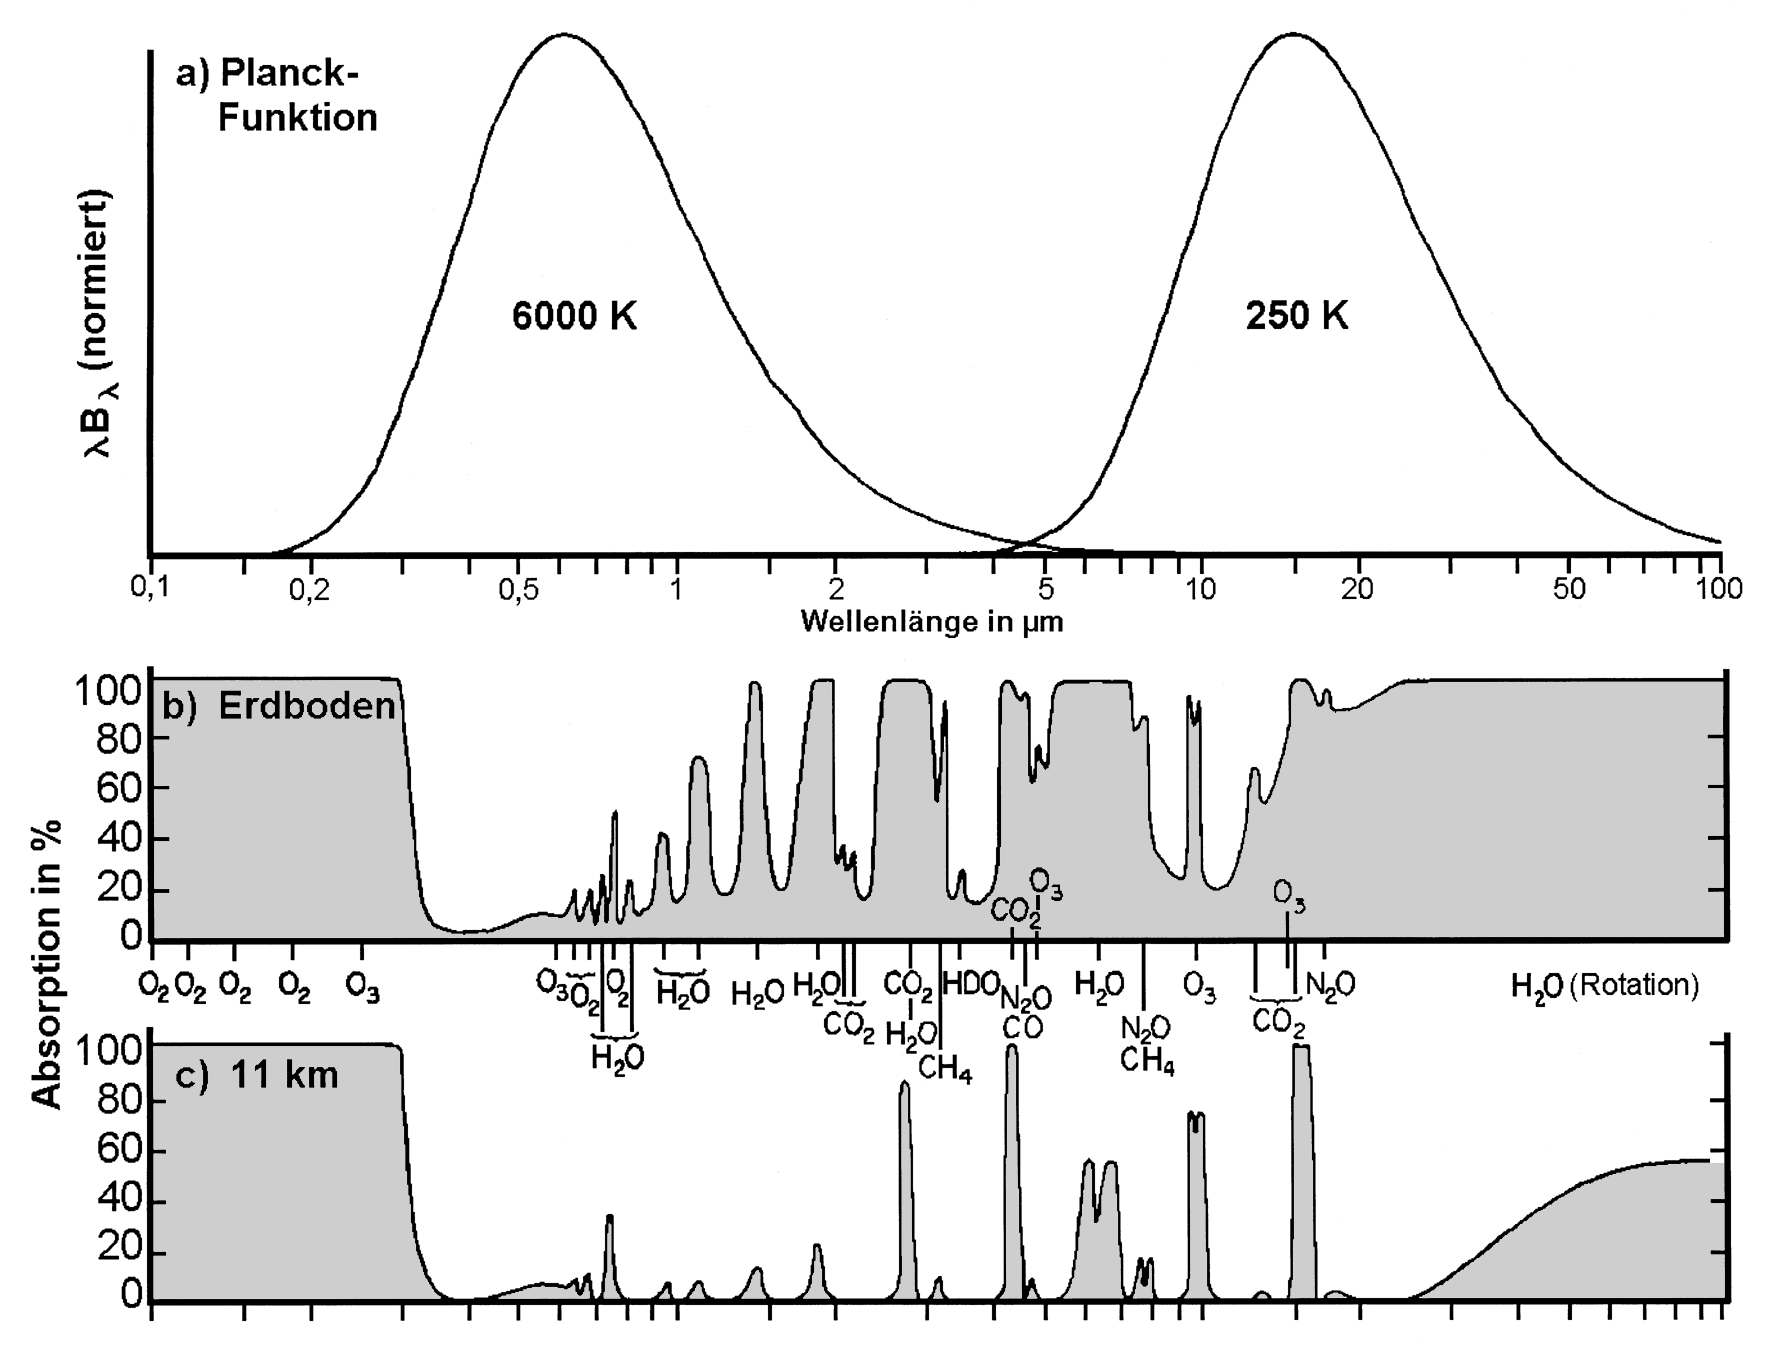
\includegraphics[width=0.7\textwidth]{../media/B1.1/Spektrum_Sonne_Erde.png}
	\caption{Spektrum der als Schwarzkörper idealisierten Sonne\\
		sowie der Erde mit logarithmischer Wellenlängenskala $\mathrm a)$,\\
		und das Absorbtionsvermögen auf der Erdoberfläche $\mathrm b)$\\
		sowie $11\mathrm{\,km}$ oberhalb der Erdoberfläche $\mathrm c)$ \cite{GoodyYung}}
	\label{abb:Spektrum Sonne & Erde}
\end{figure}

\subsection{Spektroskopie}
\label{Spektroskopie}
Spektroskopie beschreibt die Wechselwirkung von Stoffen mit elektromagnetischen Wellen. Misst man solche Wechselwirkungen im Abhängigkeit von der Wellenlänge $\lambda$ bzw. Frequenz $\nu$, so erhält man ein Spektrum, was zu der Namensgebung Spektroskopie führt.

% Historisches
Isaac Newton entdeckte bereits im $17.$ Jahrhundert die Spektralfarben des Lichtes mithilfe eines Prismas. Etwa $200$ Jahre später entdeckte Joseph von Fraunhofer die Absorptionslinie im Sonnenspektrum und erkannte damit, dass Stoffe in der Atmosphäre Teile des Spektrums ``schlucken''. Diese und viele weitere Experimente führten zu einem weiten Verständnis von diesem Bereich der Atomphysik.

\subsubsection{Licht}
\label{Licht}
Ein wichtiges Konzept der Spektroskopie ist das Licht. Es kann auf zwei Arten beschrieben werden, als Welle mit einer Wellenlänge $\lambda$ bzw. Frequenz $\nu$ und als Teilchen. Dieses Lichtteilchen nennt man Photonen. Aufgrund dessen werden beide Betrachtungsweisen gemeinsam als ``Welle--Teilchen--Dualismus'' bezeichnet. Die Energie $E$ einer elektromagnetischen Welle kann durch die Frequenz $\nu$ und das Planck'sche Wirkungsquantum $h$ beschrieben werden, das Verhältnis zwischen Frequenz und Wellenlänge durch die Lichtgeschwindigkeit $c$

\begin{eqnarray}
	E &=& h \cdot \nu \\
	c &=& \nu\lambda \\
	h &\approx& 6.63 \cdot 10^{-34} \mathrm{\,Js}
\end{eqnarray}

\hypertarget{elektromagnetisches-spektrum}{\subsection{elektromagnetisches Spektrum}\label{elektromagnetisches-spektrum}}
Das elektromagnetische Spektrum umfasst alle elektromagnetischen Wellen, die aus zueinander senkrecht stehenden elektrischen und magnetischen Wellen bestehen. Jede Wellenart besitzt eine charakteristische Wellenlänge und Frequenz bzw. Energie.

Zu dem Spektrum gehören unter anderem Radiowellen, Infrarotstrahlung, sichtbares Licht, UV--Strahlung und Gamma--Strahlung. Abbildung \ref{abb:EM Spektrum} zeigt das gesamte elektromagnetische Spektrum und die dazugehörige Wellenlängen und Frequenzen.

Dieser Versuch beschäftigt sich mit der Infrarot-- bzw. Wärmestrahlung. Ihr Bereich umfasst die Wellenlängen von $780\mathrm{\,nm}$ bis $1\mathrm{\,nm}$.

\begin{figure}[h!]
	\centering
	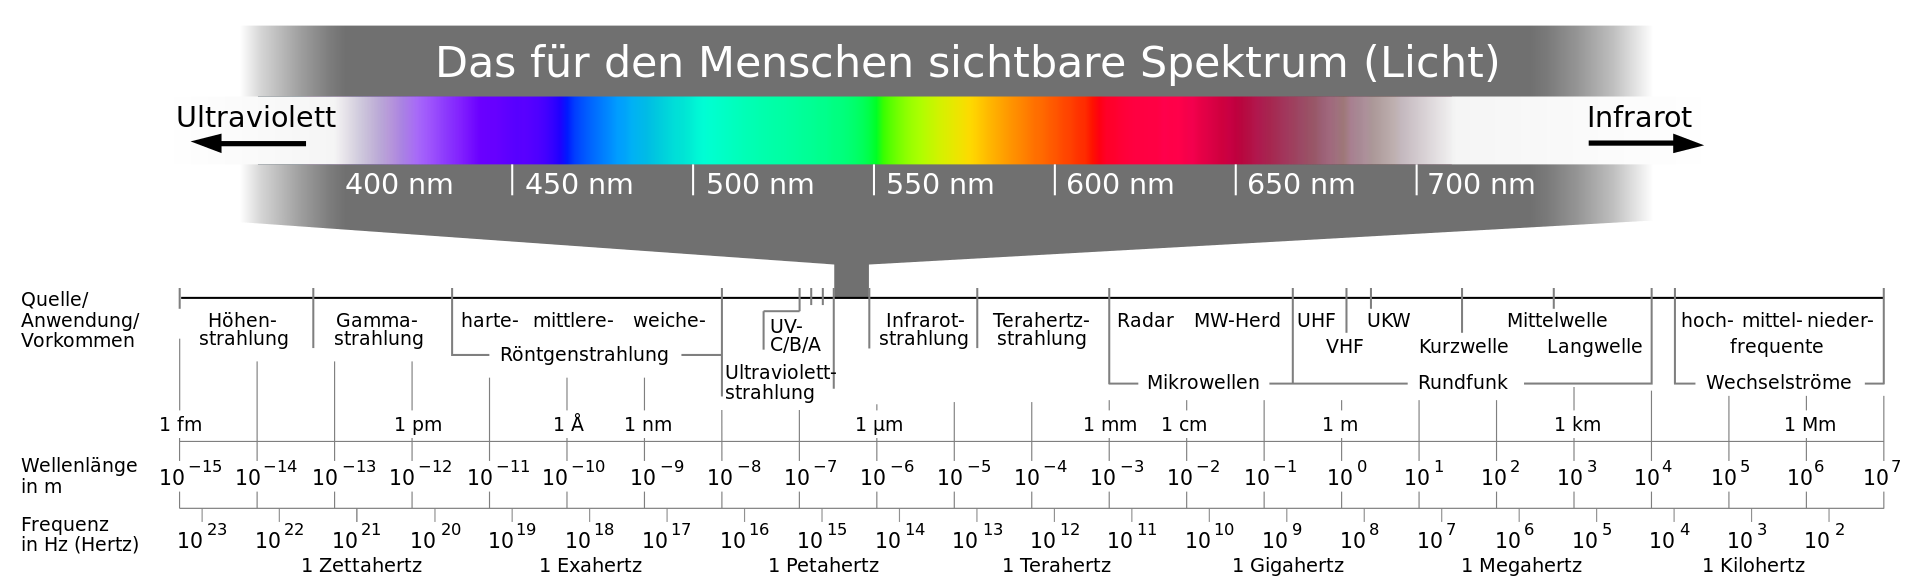
\includegraphics[width=0.7\textwidth]{../media/B1.1/EM_Spektrum.png}
	\caption{Elektromagnetisches Spektrum \cite{Wikipedia: Elektromagnetisches Spektrum}}
	\label{abb:EM Spektrum}
\end{figure}

\subsubsection{Übergänge}
\label{Übergänge}
Es gibt zwei Prozesse der Wechselwirkung mit elektromagnetischer Strahlung. Bei der \emph{Absorption} wird Energie aufgenommen, bei der \emph{Emission} wird sie abgegeben. Hierbei treten Übergänge zwischen verschiedenen Energiezuständen auf. Energiedifferenzen zwischen diesen Energieniveaus variieren. Nur wenn die Energie des Photon exakt der Energiedifferenz entspricht, kann ein Übergang stattfinden.

In der Atomschale hat man unter anderem Elektronenzustände, Schwingungszustände und Rotationszustände mit $\Delta E_{e} > \Delta E_{s} > \Delta E_{r}$ \cite{Agilent Technologies}. Die Schwingungs-- und Rotationsenergien liegen im Bereich der Infrarotstrahlung, daher sind sie für diesen Versuch relevant. Abbildung \ref{abb:Übergänge} zeigt die verschiedene Energiezustände sowie Elektronenübergänge, die mittels UV--Strahlungs--Absorption stattfinden.

Wie ein System aus Atomen das Licht absorbiert, hängt von quantenmechanischen Eigenschaften ab, die von sogenannten \emph{Auswahlregeln} beschrieben. Daraus kann man dann Rückschlüsse über das System ziehen.

\begin{figure}[h!]
	\centering
	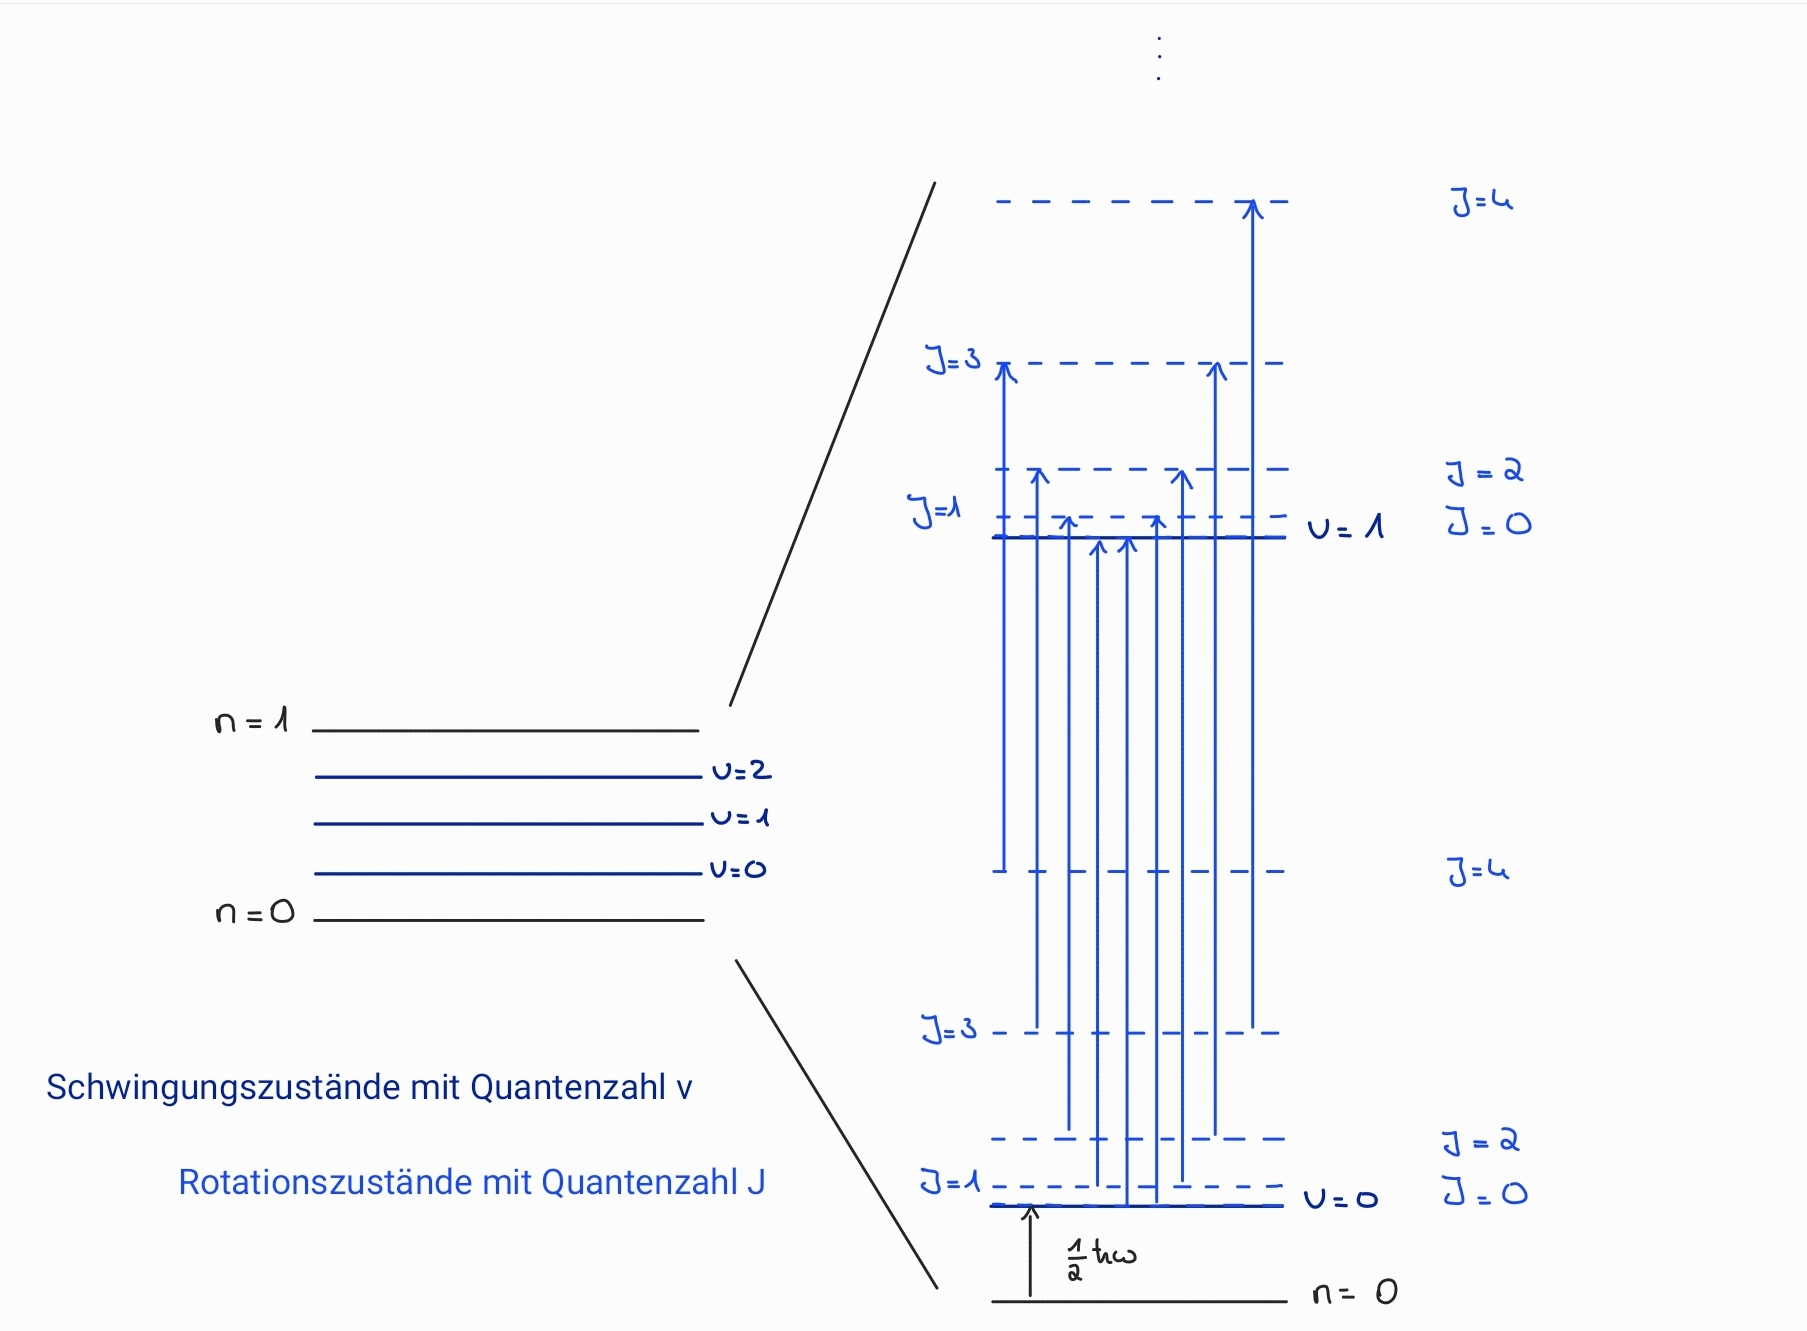
\includegraphics[width=0.7\textwidth]{../media/B1.1/Uebergaenge.jpg}
	\caption{Energiezustände und Elektronenübergang \cite{Agilent Technologies}}
	\label{abb:Übergänge}
\end{figure}

\subsubsection{Auswahlregeln}
Die Auswahlregeln beschreiben, welche Übergänge erlaubt oder verboten sind. Sie basieren auf den Erhaltungssätzen und quantenmechanischen Eigenschaften.

Beispielsweise besitzen Elektronen einen Spin von $\pm\frac{1}{2}$ und Photonen einen Spin von $1$. Daher kann ein Elektron nur dann zwischen zwei Energieniveaus wechseln, wenn sein Spin um $1$ verändert wird. Da das Photon beim Übergang entweder erzeugt oder vernichtet wird, ist der Gesamtspin auf diese Weise erhalten.

\hypertarget{planckstrahlung}{%
\subsection{Planck--Strahlung}\label{planckstrahlung}}

Das Planck'sche Strahlungsgesetz beschreibt die Energiedichte $\omega_\mathrm{P}$, die ein schwarzer Körper mit einer Frequenz $\nu$ bei einer Temperatur $T$ als Wärmestrahlung aussendet. Dabei finden das Planck'sche Wirkungsquantum $h$, die Lichtgeschwindigkeit $c$ und die Boltzmann--Konstante $k_B$ Verwendung. \cite{Demtröder Atom}

\begin{eqnarray}
    \omega_\mathrm{P}(\nu,T) &=&
        \frac{8\pi\nu^2}{c^3}
        \frac{h\nu}{\exp\left[\frac{h\nu}{k_BT}\right]-1}
        \,\mathrm d\nu
        \label{eq:PlackStrahlung}
\end{eqnarray}

\noindent
Der Faktor $\frac{8\pi\nu^2}{c^3}$ ist dabei die Dichte der Schwingungsmoden in einem Frequenzintervall, also die Anzahl erlaubter Schwingungszustände. Der Faktor $h\nu\cdot\exp[\dots]^{-1}$ beschreibt die mittlere kinetische Energie dieser Zustände. Dies ist in Abbildung \ref{abb:SpektrumSK} dargestellt.

\begin{figure}[h!]
	\centering
	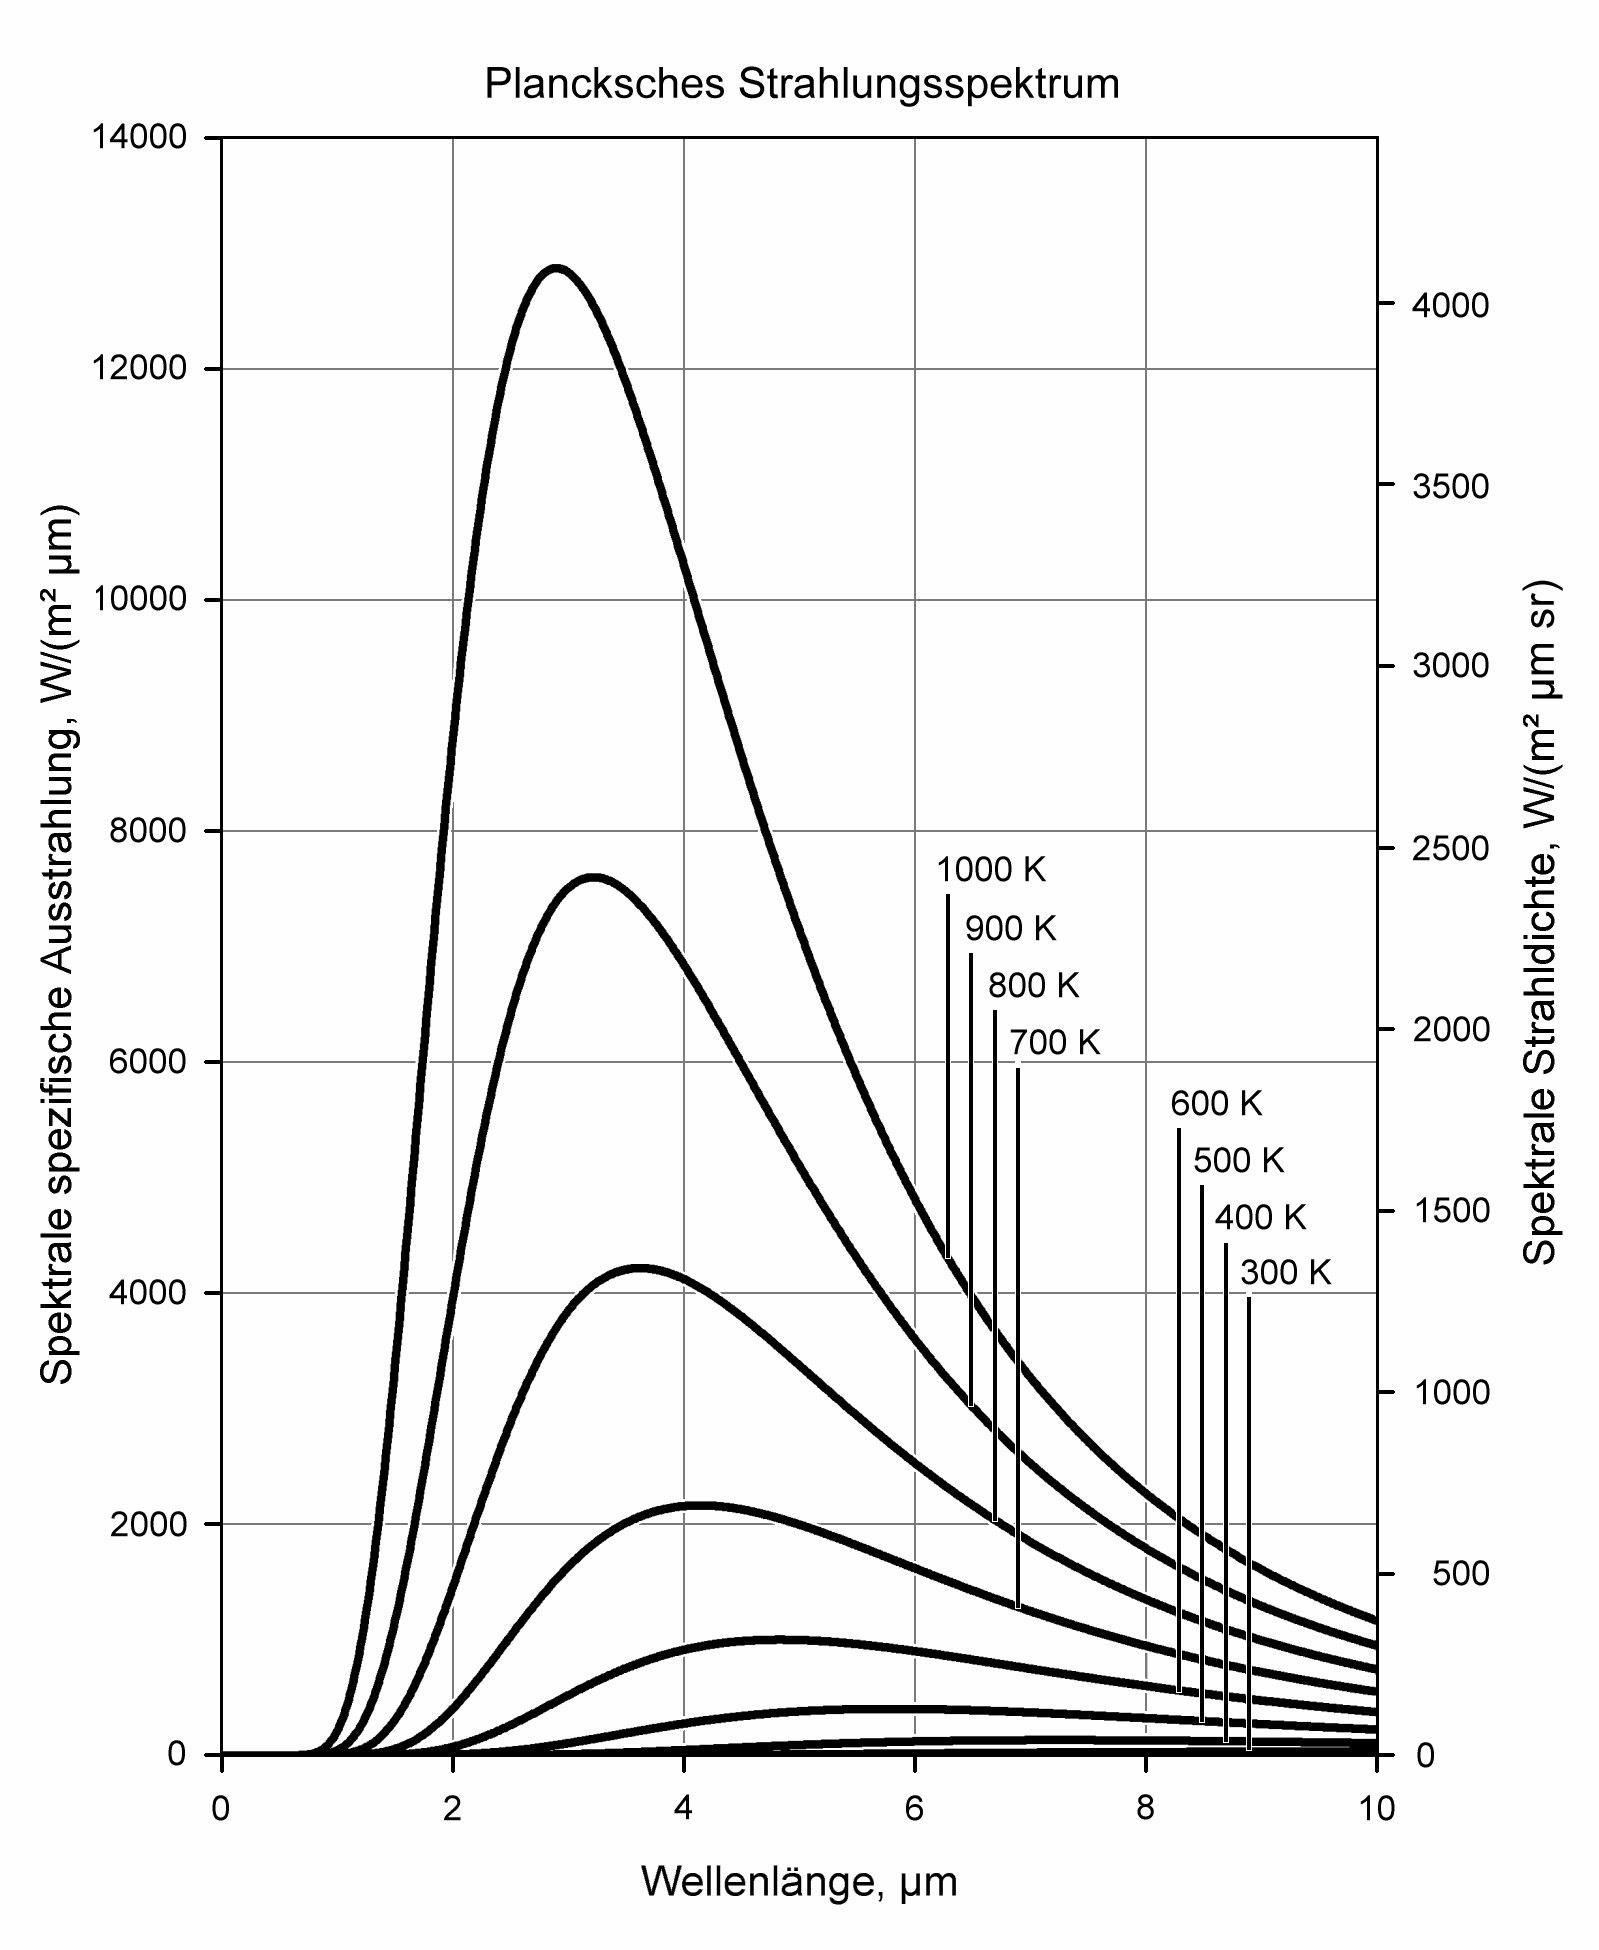
\includegraphics[width=0.5\textwidth]{../media/B1.1/BlackbodySpectrum_lin_150dpi_de.png}
	\caption{Schwarzkörperstrahlung für verschiedene Temperaturen \cite{abb:SpektrumSK}}
	\label{abb:SpektrumSK}
\end{figure}

\hypertarget{strahlungsdichte}{%
\subsubsection{Strahlungsdichte}\label{strahlungsdichte}}

Die Strahldichte oder Strahlungsdichte $S$ beschreibt die Strahlung, die ein Flächenelement $\mathrm dA$ eines Strahlers in einen Raumwinkel $\mathrm d\Omega$ abstrahlt. Sie ist allgemein das Differential der Strahlungsleistung $\Phi$. \cite{Demtröder Atom,Strahldichte}

\begin{eqnarray}
    S &=& \frac{\mathrm d^2\Phi}{\mathrm dA \cdot \mathrm d\Omega}
\end{eqnarray}

\hypertarget{wiensches-verschiebungsgesetz}{%
\subsubsection{Wien'sches Verschiebungsgesetz}\label{wiensches-verschiebungsgesetz}}

Das Wien'sche Verschiebungsgesetz beschreibt abhängig von der Temperatur $T$, bei welcher Wellenlänge $\hat{\lambda}$ bzw. Frequenz $\hat{\nu}$ die größte Wärmeleistung abgestrahlt wird. Dadurch beschreibt es die Temperaturabhängigkeit des Maximums des Planck'schen Strahlungsgesetzes $\eqref{eq:PlackStrahlung}$.

\begin{eqnarray}
    \hat{\lambda}\cdot T &=& 2.898 \cdot \mathrm{\,mm\cdot K}
        \label{eq:WienLambda}\\
    \hat{\nu}\cdot T &=& 5.879\cdot10^{10} \mathrm{\,m\cdot Hz}
        \label{eq:WienNu}
\end{eqnarray}

\hypertarget{elektrisches-dipolmoment}{%
\subsection{elektrisches Dipolmoment}\label{elektrisches-dipolmoment}}

Das elektrische Dipolmoment $\vec \mu$ ist das erste Moment aus der Multipolentwicklung einer Ladungsverteilung $\rho(\vec r)$. \cite{Dipolmoment} Es ist parallel zum elektrischen Feld $\vec E$ und beschreibt die Ungleichverteilung von Ladungen.

\begin{eqnarray}
    \vec \mu &=& \int \vec r \rho(\vec r) \,\mathrm d^3\vec r
\end{eqnarray}

\noindent
Atome im Grundzustand haben kein permanentes Dipolmoment, Moleküle können dagegen ein permanentes Dipolmoment haben. Ein Beispiel dafür ist Wasser $(\ce{H_2O})$.

\hypertarget{dipoluxfcbergang}{%
\subsubsection{Dipolübergang}\label{dipoluxfcbergang}}

Um ein Molekül durch die Absorption eines Photons anzuregen, muss ein Dipolübergang stattfinden. Dabei wird der quantenmechanische Zustand des Moleküls gestört, was durch zeitabhängige Störungstheorie beschrieben wird. \cite{Hinderer}

Dipolübergänge sind \emph{erlaubte Übergänge}. Im Unterschied dazu gibt es auch \emph{verbotene Übergänge}. Diese sind Multipolübergänge höherer Ordung und treten daher sehr viel weniger wahrscheinlich auf.

\hypertarget{uxfcbergangsdipolmoment}{%
\subsubsection{Übergangsdipolmoment}\label{uxfcbergangsdipolmoment}}

Die Störung wird als Übergangsdipolmoment $\vec\mu_{01}$ bezeichnet. Es wird durch den Operator des Dipolmoments $\hat {\vec \mu}_e$ sowie den Anfangszustand $\ket{\Psi_0}$ und den Endzustand $\ket{\Psi_1}$ berechnet. So lange das Übergangsdipolmoment $\vec\mu_{01}\neq0$ nicht verschwindet, ist der Übergang erlaubt.

\begin{eqnarray}
    \vec \mu_{01} &=& \expval{\Psi_0\left|\hat {\vec \mu}_e\right|\Psi_1}
\end{eqnarray}

\noindent
Je größer das Übergangsdipolmoment ist, desto großer ist auch das Absorptionsvermögen.

\hypertarget{freiheitsgrade}{%
\subsection{Freiheitsgrade}\label{freiheitsgrade}}

Freiheitsgrade beschreiben in der Mechanik die unabhängigen, verallgemeinerten Koordinaten eines Systems, beispielsweise eines einzelnen Atoms oder eines Moleküls.

Ein freies einatomiges Molekül besitzt drei Translationsfreiheitsgrade $f_\mathrm{trans}$, denn es kann sich frei in drei Raumrichtungen bewegen. \cite{Gerthsen}

Ein mehratomiges Molekül hat zusätzlich noch drei weitere Rotationsfreiheitsgrade $f_\mathrm{rot}$, denn es gibt zwei Rotationsachsen senkrecht zu Bindungsrichtung und einen um die Bindungsachse. Die Bewegung um die Bindungsachse ist bei bei linearen Molekülen jedoch stark eingeschränkt, dieser Freiheitsgrad ist somit verschwindend gering. \cite{Freiheitsgrad} Ein gewinkeltes Molekül wie das Wassermolekül besitzt dagegen alle drei Rotationsfreiheitsgrade. \cite{Gerthsen}

Ist ein Molekül schwingungsfähig, so muss man zudem noch Vibrationsfreiheitsgrade $f_\mathrm{vib}$ berücksichtigen. Besonders wenn sich das Molekül in einer Gitterstruktur befindet, kann es nicht wirklich rotieren, aber trotzdem in drei Raumrichtungen schwingen. Dadurch hat es sechs Freiheitsgrade, jeweils drei aus der kinetischen und der potentiellen Energie.

Ein System aus $N$ ungekoppelten Massenpunkten hat allgemein $3N$ Freiheitsgrade, wobei $f_\mathrm{vib}$ folgendermaßen bestimmt wird. \cite{Gerthsen}

\begin{eqnarray}
	 f_\mathrm{vib} &=& 3N - (f_\mathrm{trans} + f_\mathrm{rot})
\end{eqnarray}

\subsubsection{Normalschwingungen}
\label{Normalschwingungen}

Normalschwingungen sind Schwingungen, bei denen das Molekül sich mit konstanter Frequenz aus einer Ruhelage bewegt, wobei Gesamtimpuls und Gesamtdrehimpuls erhalten bleiben.

Da es immer eine longitudinale und zwei transversale Schwingungsrichtungen gibt, ist die Anzahl der Normalschwingungen immer ein Vielfaches von $3$. \cite{Gerthsen}

Beispielsweise hat Kohlenstoffdioxid $\ce{CO_2}$ drei Normalschwingungen, die in Abbildung \ref{abb:Normalschwingungen CO2} dargestellt sind. Die symmetrische und antisymmetrische Streckschwingung unterscheiden sich qualitativ. Die Biegeschwingungen dagegen sind entartet und bilden daher denselben Vibrationsfreiheitsgrad.

\begin{figure}[h!]
	\centering
	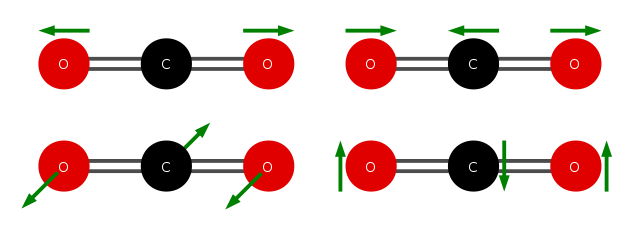
\includegraphics[width=0.7\textwidth]{../media/B1.1/Normalschwingung_CO2.png}
	\caption{Normalschwingungen von $\ce{CO_2}$ \cite{abb:Schwingungen CO2}\\
		oben: Streckschwingungen, (links symmetrisch, rechts antisymmetrisch)\\
		unten: Biegeschwingungen in zwei Entartungen}
	\label{abb:Normalschwingungen CO2}
\end{figure}

\subsubsection{Rotationsniveaus}
Ein rotierendes zweiatomiges Molekül lässt sich als linearer starrer Rotor betrachten.

Seine quantenmechanischen Energieniveaus $E_J$ sind durch den Eigenwert des Drehimpulsoperators $\hat J$ und die Rotationskonstante $\tilde{B}$ bestimmt. $\tilde{B}$  wiederum wird durch das Trägheitsmoment $I$ und das reduzierte Plank'sche Wirkungsquantum $\hbar$ dargestellt.

\begin{eqnarray}
	E_J &=& \tilde{B} J (J + 1) \\
	\tilde{B} &=& \frac{\hbar^2}{2 I}
\end{eqnarray}

\noindent
Typische Frequenzen für die Rotationsanregung bei Molekülen befinden sich im sub--millimeter--Bereich, wobei sie sich für die Vibrationsanregung durch Infrarotanregung. % \cite[S. 4]{UzK}

\hypertarget{infrarotaktivituxe4t}{\subsubsection{Infrarotaktivität}\label{infrarotaktivituxe4t}}
Wird das elektrische Dipolmoment eines Moleküls bei einer Schwingung periodisch verändert, so wird von einer infrarot--aktiven (IR-aktiven) Schwingung gesprochen.

Das $\ce{CO_2}$--Molekül besitzt zwei  IR--aktive Normalschwingungen, die Biegeschwingung und die asymmetrische Streckschwingung.\footnote{Vergleiche Abschnitt \ref{Normalschwingungen}} Bei beiden Schwingungen wird die Symmetrie gebrochen und es ergibt sich ein periodisch veränderndes Dipolmoment.

Durch diese Schwingungen ist es möglich, $\ce{CO_2}$--Dipolübergänge im Infrarotbereich anzuregen, obwohl das $\ce{CO_2}$--Molekül  in Ruhe kein elektrisches Dipolmoment besitzt. \cite{HakenWolf} % \cite[S. 197]{HakenWolf}

\hypertarget{Rotationsbande}{\subsubsection{Rotationsbande}\label{Rotationsbande}}
In Abbildung \ref{fig:rotationsspektrumCO2} ist das Rotationsspektrum von CO$_2$ dargestellt, das bei einem Probendruck von einigen $\mathrm{\mu bar}$ aufgenommen wurde. Ein solches Spektrum wird auch \emph{Rotationsbande} genannt.

\begin{figure}[h]
	\centering
	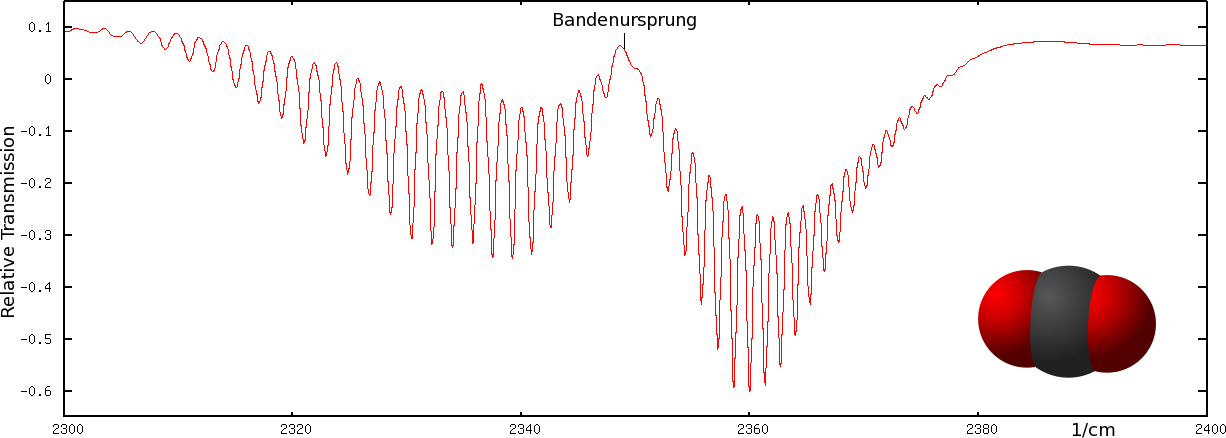
\includegraphics[width=0.7\textwidth]{../media/B1.1/Rotationssprektrum_CO2.png}
	\caption{Rotationsspektrum von $\ce{CO_2}$ bei einem Probendruck von einigen $\mathrm{\mu bar}$,\\
		gemessen mit einem FTIR--Spektrometer \cite{UzK}}
	\label{fig:rotationsspektrumCO2}
\end{figure}

Dieses lässt sich in einen P--Zweig (links) und in einen R--Zweig (rechts) aufteilen. Der P--Zweig beschreibt dabei die Auswahlregel $\Delta J = -1$ und der R--Zweig $\Delta J = +1$. Jede einzelne Linie im Spektrum stellt dann die Werte für $J$ dar, angefangen bei $0$ vom Bandenursprung nach außen hin zunehmend.

Die Intensität jeder Linie hängt stark von $J$ ab und folgt der Boltzmann--Statistik. Das erklärt die unterschiedlichen Höhen der einzelnen Linien.

Wird der Probendruck erhöht, erfolgt eine starke Linienverbreitung. Die einzelnen Linien folgen dann der Gestalt einer Lorentz--Kurve, die in Abbildung \ref{abb:Druckverbreiterung & Sättigungsverbreiterung} links dargestellt ist. Bei Zimmertemperatur beträgt der Druckverbreiterungskoeffizient ca. $0.3 \mathrm{\, cm^{-1}\cdot bar^{-1}}$. \cite{UzK}

Außerdem erfolgt eine Sättigungsverbreiterung bei höheren Konzentrationen von $\ce{CO_2}$. So erscheinen die Linien bei hohen Konzentrationen in Form einer Gauß--Glocke, wie es in Abbildung \ref{abb:Druckverbreiterung & Sättigungsverbreiterung} rechts zu sehen ist. Dieses Verhalten entsteht durch den Einfluss des im Folgenden besprochenen Lambert--Beer'schen Gesetzes für zunehmende Konzentration.

\begin{figure}[h]
	\centering
	\begin{minipage}{0.49\textwidth}
		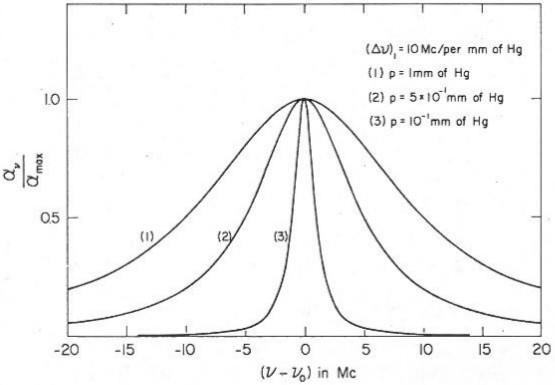
\includegraphics[width=\textwidth]{../media/B1.1/Druckverbreiterung.jpg}
	\end{minipage}
	\begin{minipage}{0.49\textwidth}
		\includegraphics[width=\linewidth]{../media/B1.1/Sättigungsverbreiterung.jpg}
	\end{minipage}
	\caption{Druckverbreiterung (links) und Sättigungsverbreiterung (rechts) \cite{UzK}}
	\label{abb:Druckverbreiterung & Sättigungsverbreiterung}
\end{figure}

\hypertarget{das-lambertbeersche-gesetz}{\subsubsection{Das Lambert--Beer'sche Gesetz}\label{das-lambertbeersche-gesetz}}
Das Lambert--Beer'sche Gesetz beschreibt die transmittierte Intensität $I$ in Abhängigkeit der eintreffenden Intensität $I_0$. \cite{HakenWolf} % \cite[S. 299f]{HakenWolf}

\begin{eqnarray}
	I &=& I_0 e^{- \alpha C x} \label{eq:Lambert-Beer}
\end{eqnarray}

\noindent
Dabei sind der für jedes Molekül charakteristische Absorptionskoeffizient $\alpha$ , die Konzentration $C$ der absorbierenden Moleküle in einer homogenen Probe und die Dicke $x$ dieser Probe relevant.

Mithilfe dieses Gesetzes lässt sich die Lambert--Beer--Gauß--Formel \eqref{eq:Lambert-Beer-Gauß} herleiten. Sie entsteht, wenn die gesamte transmittierte Intensität $I(C)$ von eintreffenden elektromagnetischen Wellen aller Frequenzen im Intervall $[\nu_1, \nu_2]$ gesucht wird.

Diese Formel ergibt sich aus dem Integral über das Lambert--Beer'sche Gesetz, wobei die Frequenzabhängigkeit des Absorptionskoeffizienten $\alpha(\nu)$ relevant ist. Dafür wird hier eine Gauß--Verteilung angenommen,

\begin{eqnarray}
	%I(C) &=& I_0 \int_{\nu_1}^{\nu_2} \exp[-\alpha(\nu^\prime) C x] \,\mathrm d\nu^\prime \\
	\alpha(\nu) &=& \alpha_0 \exp[- \left(\frac{\nu - \nu_0}{\Delta \nu}\right)^2] \\
	I(C) &=& I_0 \int_{\nu_1}^{\nu_2} \exp[-\alpha_0 \exp \left[- \left(\frac{\nu' - \nu_0}{\Delta \nu}\right)^2\right] C x] d\nu' \label{eq:Lambert-Beer-Gauß}
\end{eqnarray}

\subsection{pyroelektrischer Sensor}
Ein pyroelektrischer Sensor wandelt Temperaturunterschiede durch den \emph{pyroelektrischen Effekt}\footnote{verwandt mit dem piezoelektrischen Effekt} in Spannungen um.

Ein solcher Sensor besteht aus zwei Elektroden und einer Schicht aus pyroelektrischem Material. Das Kristallgitter eines pyroelektrischen Materials besitzt zwei Arten von Gitterschichten, jeweils eine ist mit positiven und eine mit negativen Ionen besetzt. \cite{pyroelektrischer Sensor}

Wenn Infrarotstrahlung absorbiert wird, führt dies zu einer lokalen Verformung des Gitters, wodurch sich die Abstände zwischen positiven und negativen Ionen verändern. Dann fällt eine messbare Spannung über die Elektroden ab.

\begin{figure}[h!]
	\centering
	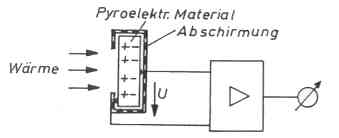
\includegraphics[width=0.5\textwidth]{../media/B1.1/IR_Sensor.jpg}
	\caption{Schematisches Prinzip eines IR--Detektors \cite{pyroelektrischer Sensor}}
	\label{abb:pyroelektrischer Sensor}
\end{figure}

\hypertarget{mathematische-grundlagen}{%
\subsection{Mathematische Grundlagen}\label{mathematische-grundlagen}}

\hypertarget{gauuxdfverteilung}{%
\subsubsection{Gaußverteilung}\label{gauuxdfverteilung}}

Die Gaußverteilung entspricht der Wahrscheinlichkeitsdichtefunktion $\phi_{\mu,\sigma^2}(\chi)$ mit dem Erwartungswert $\mu$ und der Standardabweichung $\sigma$. Manchmal wird die Gaußverteilung auch als Normalverteilung bezeichnet, manchmal bezeichnet die Normalverteilung dagegen einen Spezialfall mit $\mu=\sigma=1$. In Abbildung \ref{abb:gaussians} sind verschiedene Gaußverteilungen dargestellt.

\begin{eqnarray}
    \phi_{\mu,\sigma^2}(\chi) &=&
        \frac{1}{\sqrt{2\pi\sigma^2}}
        \exp\left[
            -
            \frac{(\chi - \mu)^2}{2\sigma^2}
        \right]
\end{eqnarray}

\noindent
Werden Zufallsvariablen gemessen, so haben sie immer eine gewisse Streuung. Nach dem Grenzwertsatz ist diese Streuung gaußverteilt. Bei genügend Messungen kann man annehmen, dass $68.3\%$ der Zufallsvariablen im Intervall $\mu\pm\sigma$ liegen.

Im $2\sigma$--Intervall werden $95.4\%$ der Zufallsvariablen erwartet, im $3\sigma$--Intervall sogar $99.7\%$.

\begin{figure}[h]
	\centering
	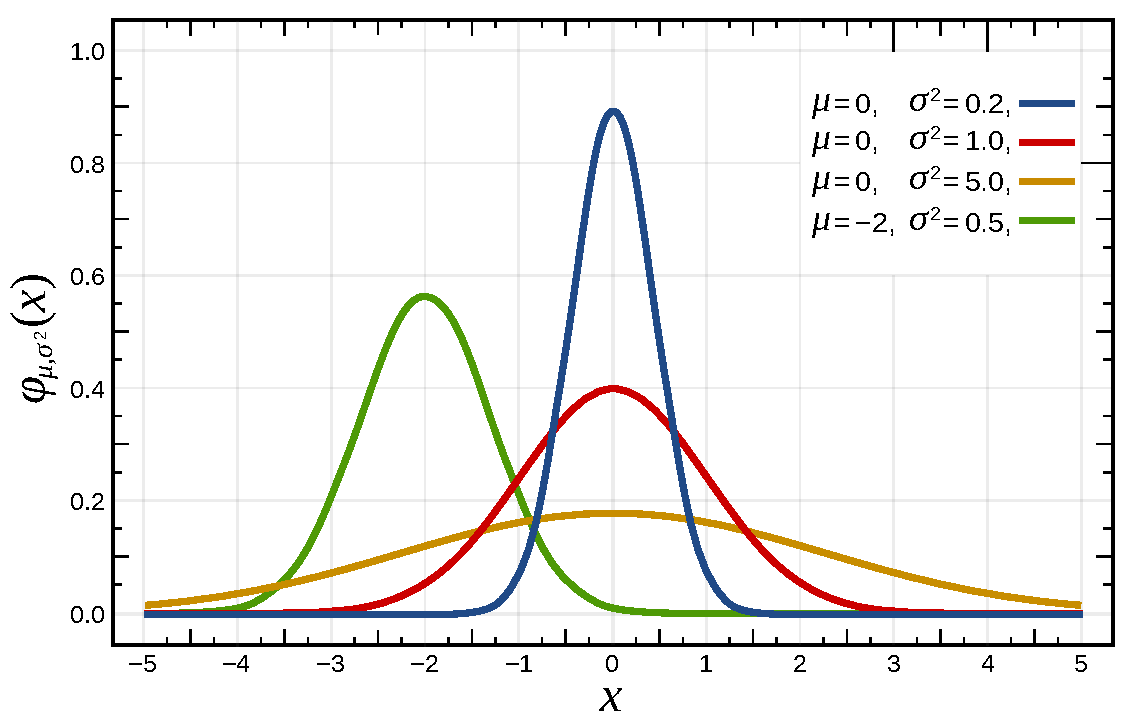
\includegraphics[width=0.7\textwidth]{../media/B1.1/Gaussverteilungen.pdf}
	\caption{Gaußverteilungen mit verschiedenen Parametern \cite{abb:gaussians}}
	\label{abb:gaussians}
\end{figure}

\hypertarget{treppenfunktion}{%
\subsubsection{Treppenfunktion}\label{treppenfunktion}}

Eine Treppenfunktion ist eine Funktion, die abschnittsweise aus konstanten Funktionen zusammengesetzt ist.

Sei $\tau:[a,b]\rightarrow \mathbb R$ eine Treppenfunktion, dann gibt es $N$ Intervalle $(x_i, x_{i+1})$ und Konstanten $c_i$, sodass folgende Bedingungen erfüllt sind. \cite{Einsiedler}

\begin{eqnarray}
    x_0 &=& a \\
    x_n &=& b \\
    \forall i:\quad
        x_i &<& x_{i+1} \\
    \forall x\in[x_i, x_{i+1}]:\quad
        \tau(x) &=& c_i
\end{eqnarray}

\noindent
Das Integral über eine Treppenfunktion wird als Summe über die Zerlegung $\{x_i\}$ gebildet.

\begin{eqnarray}
    \int_a^b\tau(x)\,\mathrm dx
        &=& \sum_{i=0}^N c_i\cdot (x_{i+i}-x_i)
\end{eqnarray}

\hypertarget{numerische-integration}{%
\subsubsection{numerische Integration}\label{numerische-integration}}

Ein Integral $\int_a^b f$ kann numerisch angenähert werden, indem die Funktion $f$ durch eine Treppenfunktion dargestellt wird. Diese Methode addiert rechteckige Flächenelemente, es gibt auch ähnliche Methoden mit beispielsweise trapezförmigen Flächenelementen.

Der Integrationsbereich $[a,b]$ wird in $N$ gleich große Intervalle zerlegt. Dadurch kann die Schrittweite $\Delta x$ definiert werden. Die Stufenfunktion wird so gewählt, dass die Funktion $f$ in jedem Teilintervall $(x_i, x_{i+1})$ angenähert wird. Damit kann das Integral ermittelt werden.

\begin{eqnarray}
    \Delta x &=& \frac{b--a}{N} \\
    \forall i:\quad
        f(x) &\approx& f(x+i\cdot\Delta x) \\
    \int_a^b f(x) \,\mathrm dx
        &\approx& \Delta x\cdot
            \sum_{i=1}^N f(x + i\cdot \Delta x)
\end{eqnarray}

\noindent
Dies ist nur eine Annäherung eines echten Integrals, die kein exaktes Ergebnis liefert. Wenn $\Delta x$ beliebig klein werden könnte, so nähert man sich einem Riemann--Integral an.

\hypertarget{gewichteter-mittelwert}{%
\subsubsection{gewichteter Mittelwert}\label{gewichteter-mittelwert}}

Ein Mittelwert von $n$ Werten $x_i$ kann beliebig mit Gewichten $w_i$ manipuliert werden.

Sind die Gewichte $w_i$ nicht normiert, d.h. $\sum_{i=1}^n w_i\neq 1$, so muss die gewichtete Summe durch die Summe der Gewichte geteilt werden, um den gewichteten Mittelwert zu erhalten.

Haben die Einzelwerte $x_i$ eigene Ungenauigkeiten $\Delta x_i$, wie beispielsweise Messungenauigkeiten, kann man den inversen Fehler als Gewicht verwenden. Der so gewichtete Mittelwert hat dem normalen Mittelwert gegenüber den Vorteil, dass die Werte mit einem größeren Fehler weniger stark einfließen als die mit geringerem Fehler. Die Ungenauigkeit des Mittelwertes $\Delta \bar x$ wird durch die Mittlere Quadratsumme der Residuen bestimmt.

\begin{eqnarray}
    \bar{x} &=&
        \frac{\sum_{i=1}^n w_i x_i}{\sum_{i=1}^n w_i}\\
    w_i &=& \frac{1}{(\Delta x_i)^2}
\end{eqnarray}

\hypertarget{mittlere-quadratsumme-der-residuen}{%
\subsubsection{Mittlere Quadratsumme der Residuen}\label{mittlere-quadratsumme-der-residuen}}

Die Mittlere Quadratsumme der Residuen (MQR) ähnelt der Standardabweichung. Diese ist für Messergebnisse, deren Mittelwert ermittelt wird, allerdings verzerrt, da ein statistischer Freiheitsgrad $f_S$ durch die Bildung des Mittelwertes verloren geht. Bei der linearen Regression gehen sogar zwei Freiheitsgrade verloren.

Deswegen wird bei der MQR nicht durch die Stichprobenmenge $n$ geteilt, sondern durch die Zahl der Freiheitsgrade. Seien $y$ Freiheitsgrade gebunden gilt folgendes. Für den Mittelwert gilt beispielsweise $y=1$.

\begin{eqnarray}
    \Delta x &=& \pm\sqrt{\frac{1}{n(n - y)}\sum_{i=1}^n(\bar{x}-x_i)^2}
\end{eqnarray}

\clearpage
\hypertarget{durchfuxfchrung}{%
\section{Durchführung}\label{durchfuxfchrung}}
\subsection{Versuchsaufbau}
\label{Versuchsaufbau}

Der Versuchsaufbau besteht im Wesentlichen aus einer Infrarot--Quelle, einer Absorptionszelle mit Thermometer und einem Infrarot--Detektor. Dies ist in Abbildung \ref{abb:Aufbau} schematisch dargestellt.

Die Infrarot--Quelle ist eine metallische Drahtwendel, die näherungsweise als Schwarzer Körper anngenommen werden kann. Sie ist umgeben von einem Reflektor, sodass das Licht gebündelt in die Aparatur geleitet wird.

\begin{figure}[h!]
	\centering
	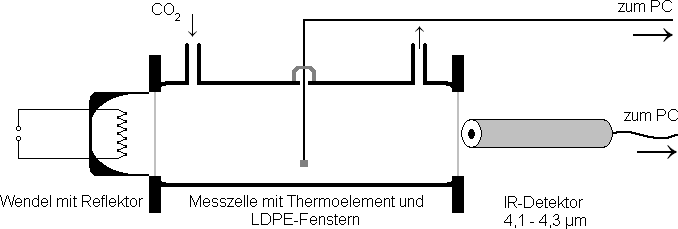
\includegraphics[width=0.7\textwidth]{../media/B1.1/IR_Aufbau.png}
	\caption{Schematische Darstellung des Aufbaus \cite{UzK}}
	\label{abb:Aufbau}
\end{figure}

Bei der Absorptionszelle handelt es sich um ein verspiegeltes Glasrohr mit zwei infrarotdurchlässigen Fenstern an jedem Ende und zwei kleinen Öffnungen für die Gaszufuhr und Entlüftung. Ein Thermometer ist mit dem Computer verbunden, um das Phänomen des Treibhauseffekts zu messen. Als Infrarot--Detektor wird ein pyroelektrischer Sensor verwendet. Die beiden Fenster bestehen aus PE--Folie.

Alle Bauteile können auf einer optischen Bank gegeneinander verschoben werden. Das Besondere an diesem Versuchsaufbau ist, dass sowohl IR--Quelle als auch IR--Detektor breitbandig sind und man spricht von Integral--Absorptionsspektrometer.

\subsection{Durchführung}
\label{durchfuehrung}
Bei dem gesamten Versuch werden die Beleuchungsstärke und die Temperatur digital gemessen. Diese Werte werden mit dem Computer aufgezeichnet und in Echtzeit als Graph dargestellt.

Zunächst schaltet man den Strom der IR--Quelle auf die maximale Stromstärke $I_\mathrm{max}\approx 8.3\mathrm{\,A}$. Dann wird die Beleuchtungsstärke so lange gemessen, bis ein nahezu konstanter, aber verrauschter Wert gemessen wird. Dies dauert in etwa $8-10\mathrm{\,min}$. Zu diesem Zeitpunkt ist ein thermisches Gleichgewicht in der Messzelle entstanden, sodass die weiteren Messungen durchgeführt werden können.

Dies entspricht dem Vorgehen im restlichen Versuch. Zunächst wird gemessen, dass ein Gleichgewichtszustand vorherrscht; daraufhin wird etwas verändert und wiederum gemessen, bis die Messwerte bis auf Rauschen konstant sind.

Daraufhin wird die IR--Transmission von verschiedenen Stoffen untersucht. Danach wird der Einfluss der Konzentration von $\ce{CO_2}$ in $\ce{N_2}$ auf den Temperaturverlauf gemessen.

\subsubsection{IR--Transmission}
\label{howto:IR--Transmission}

Daraufin wird die IR--Transmission von verschiedenen Materialien untersucht. Dazu sollen verschiedene Materialien direkt vor dem IR--Detektor plaziert werden. Die Proben sind eine PE--Folie, je eine orangene und eine violette Hochtemperatur--Filterfolie, eine Schicht eines Papiertaschentuchs und ein Stück Schreibpapier.

Dazu wird der Abstand zwischen Quelle und Detektor so eingestellt, dass die Beleuchtungsstärke ungefähr $0.9-1.0\mathrm{\,\frac{W}{m^2}}$ beträgt.

Als Erstes wird immer die Beleuchtungsstärke ohne Probe gemessen, bis diese für ca. $30\mathrm{\,s}$ bis auf Rauschen konstant bleibt. Daraufhin wird das Material in möglichst steilem Anstellwinkel an den Detektor gelehnt. Danach wird so lange gemessen, bis die Beleuchtungsstärke wieder bis auf Rauschen konstant ist.

\subsubsection{Konzentrationskalibrierung}
\label{howto:Konzentrationskalibrierung}
Nun wird der Abstand zwischen IR--Quelle und Absorptionszelle auf $1\mathrm{\,cm}$ eingestellt. Dann wird die Zelle gespült, indem sie für ca. eine halbe Minute mit Stickstoff $\ce{N_2}$ geflutet wird. Auf diese Weise wird zu Beginn jeder Messung der selbe Ausgangszustand hergestellt.

Die jeweiligen Messungen werden gestartet, während die Messzelle mit $\ce{N_2}$ geflutet ist. Es wird wieder auf einen Gleichgewichtszustand gewartet. Dann entnimmt man vorsichtig eine genaue Menge $\ce{CO_2}$ mit einer Spritze aus einer Gasflasche. Dieses Gas wird sofort in die Messzelle eingefüllt. Wenn die Messwerte wieder für $30\mathrm{\,s}$ näherungsweise konstant bleiben, wird die Messung gestoppt.

Mit dem Messprogramm werden die Mittelwerte der konstanten Beleuchtungsstärke jeweils vor und nach dem Befüllen mit $\ce{CO_2}$ bestimmt. Dann wird die Spritze wird danach abgenommen die Zelle wird wieder mit Stickstoff gespült.

Dieses Vorgehen wird mit in $1\mathrm{\,ml}$--Schritten mit $\ce{CO_2}$--Mengen von $1\mathrm{\,ml}$ bis $5\mathrm{\,ml}$ durchgeführt, ebenso mit $10\mathrm{\,ml}$, $15\mathrm{\,ml}$, $20\mathrm{\,ml}$, $30\mathrm{\,ml}$, $45\mathrm{\,ml}$ und $60\mathrm{\,ml}$ $\ce{CO_2}$. Bis zu einem Volumen von $10\mathrm{\,ml}$ kann eine feinere Spritze verwendet werden als für die restlichen Messungen.

Zuletzt wird eine weitere Messung von Beleuchtungsstärke und Temperatur durchgeführt, bei der die $\ce{CO_2}$--Konzentration $100\%$ beträgt. Dazu wird die  Gasflasche direkt an die Zelle angeschlossen ist und die Zelle langsam bis zur Sättigung mit $\ce{CO_2}$ befüllt. Danach danach wird die Flasche entfernt und die Zelle so lange gespült, bis die vorherige Beleuchtungsstärke wiederhergestellt ist.

\subsubsection{Spektrometrische Konzentrationsbestimmung}
\label{howto:Spektrometrische Konzentrationsbestimmung}
Der Raum wird etwa $1\mathrm{\,min}$ lang gelüftet. Danach werden die Fenster geschlossen und eine neue Messung wird gestartet, bis die Messwerte nahezu konstant sind. Dann wird der Auslassschlauch aus der Blubberflasche genommen und die Zelle wird durch einen Gummibalg mit Luft gefüllt, bis sich die Beleuchtungsstärke nicht mehr ändert. Die Mittelwerte für vor und nach dem Befüllen werden bestimmt. Abschließend wird die Zelle wieder gründlich mit Stickstoff geflutet.

\subsubsection{Optische Emission}
\label{howto:Optische Emission}
Zuletzt wird die optische Emission der IR--Quelle ermittelt. Hierfür wird der Raum komplett abgedunkelt und alle Geräte bis auf die IR--Quelle werden ausgeschaltet. Nun wird der Heizstrom langsam aufgedreht bis das Leuchten der Wendel gerade sichtbar wird. Diese Stromstärke wird für jeden Gruppenteilnehmer individuell bestimmt. Zusätzlich wird die maximale Stromstärke der Wendel festgehalten.

\clearpage
\hypertarget{auswertung}{%
\section{Auswertung}\label{auswertung}}
\subsection{IR--Transmission}
\label{IR--Transmission}

Zunächst werden die IR--Absorption und --Emission verschiedener Proben anhand ihrer Beleuchtungsstärke--Kurven untersucht. Dafür werden diese zunächst gegeneinander aufgetragen, siehe Abbildung \ref{abb:materialien}.

\begin{figure}[h]
	\centering
	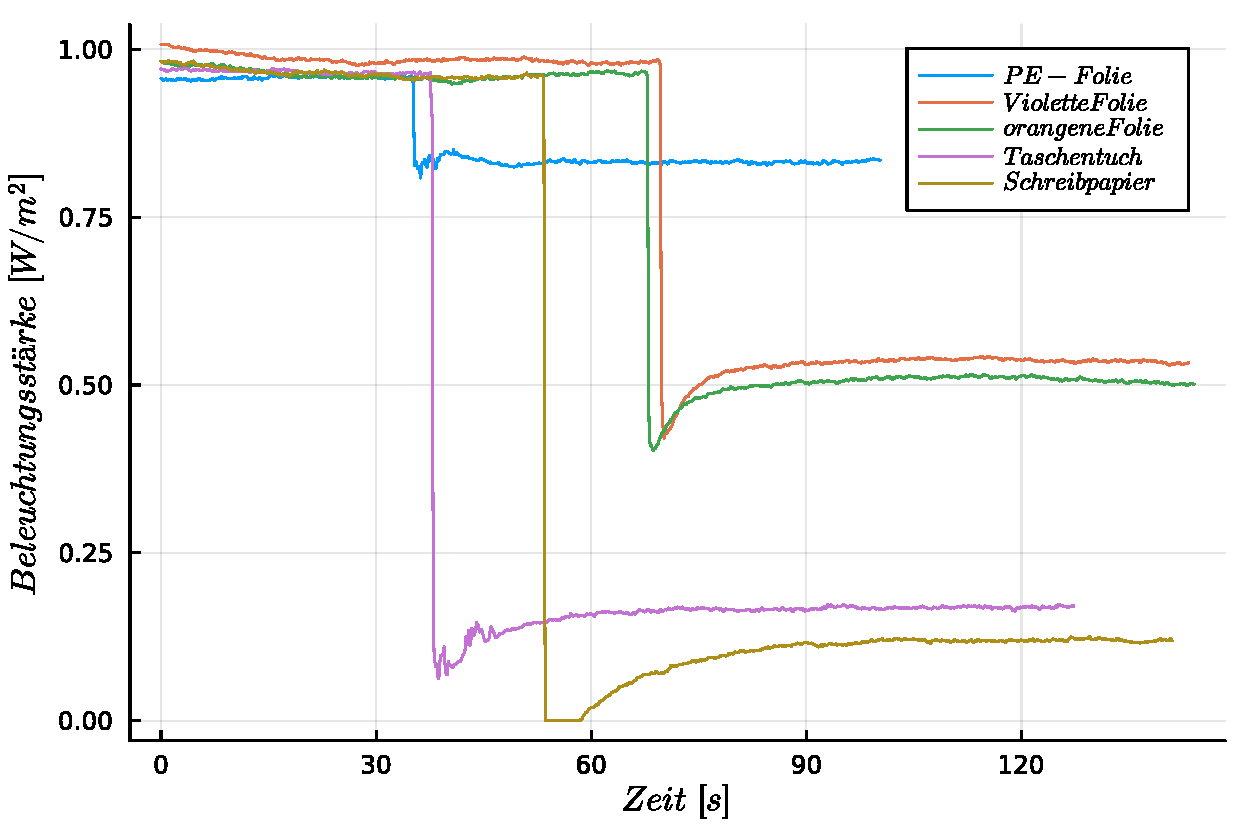
\includegraphics[width=0.7\textwidth]{../media/B1.1/materialien.pdf}
	\caption{Beleuchtungsstärke-Kurven verschiedener Proben}
	\label{abb:materialien}
\end{figure}

Der Kurvenverlauf ist allgemein für alle Proben sehr ähnlich. Solange keine Probe vor den Detektor gebracht wurde, ist die Kurve konstant. Sie fällt abrupt auf einen Minimalwert ab, wenn eine Folie vor den Detektor gestellt wird, und steigt dann langsam auf einen stationären Wert an.

Durch das Anbringen der verschiedenen Materialien zu unterschiedlichen Zeitpunkten kommt es zu einer Verschiebung der Messkurven in $x$--Richtung.

Die nicht klar definierten Minima bei der PE--Folie und dem Taschentuch lassen sich durch die Schwierigkeit beim Anbringen dieser vor dem Detektor erklären. Bei diesen dünnen Proben dauerte die Anbringung und Positionierung länger, weswegen die Messwerte schwanken. Beim Schreibpapier war kein Minimum zu sehen, da die IR--Strahlung vollkommen von diesem absorbiert wurde, dennnoch ist die Form der Kurve ähnlich zu den anderen.

Der graviserenste Unterschied zwischen den jeweiligen Messkurven sind die Höhenunterschiede zu einander. Hieraus sind klare Unterschiede im Transmissionsgrad der verschiedenen Proben su sehen. Die PE--Folie beispielsweise lässt deutlich mehr IR--Strahlung durch als das Schreibpapier.

Diese Beobachtung soll nun quantitativ untersucht werden. Dazu werden die minimalen Beleuchtungsstärken $I_\mathrm{min}$ sowie die durchschnittlichen Beleuchtungsstärken $I_\mathrm{stat}$ im stationären Bereich aus den Kurven bestimmt und jeweils die Transmissionswerte $T$ des Materials mittels der durchschnittlichen Beleuchtungsstärke ohne Material $I_0$ berechnet.

Dazu wird der Mittelwert $m$ gebildet. Der Fehler $\Delta m$ wird durch die mittlere Quadratsumme der Residuen (MQR) bestimmt. Die Ergebnisse sind in Tabelle \ref{table:materialien} dargestellt.

\begin{eqnarray}
	T &=& \frac{I}{I_0} \\
	m &=& \frac{1}{n} \sum_{i=1}^{n} x_i \\
	\Delta m &=& \sqrt{\frac{1}{n (n-1)} \sum_{i=1}^{n} (x_i - m)^2}
\end{eqnarray}

\begin{table}[h!]
	\centering
	\begin{tabular}{l|p{2.1cm}|p{2.1cm}|p{2.1cm}|p{1.8cm}|p{1.8cm}}
		Probe
			& $I_\mathrm{min}$ $[10^{-2} \mathrm{\, W/m^2}]$
			& $I_\mathrm{stat}$ $[10^{-2} \mathrm{\, W/m^2}]$
			& $I_0$ $[10^{-2} \mathrm{\, W/m^2}]$
			& $T_\mathrm{min}$ $[\%]$
			& $T_\mathrm{stat}$ $[\%]$ \\
		\hline
		PE--Folie
			& $80.8350$
			& $83.213$
			& $95.797$
			& $84.382$
			& $86.864$ \\
			& $\quad\pm 0.0005$
			& $\quad\pm 0.009$
			& $\quad\pm 0.014$
			& $\quad\pm 0.012$
			& $\quad\pm 0.015$ \\
		Violette Folie
			& $42.0750$
			& $53.625$
			& $98.338$
			& $42.786$
			& $54.532$ \\
			& $\quad\pm 0.0005$
			& $\quad\pm 0.012$
			& $\quad\pm 0.014$
			& $\quad\pm 0.006$
			& $\quad\pm 0.014$ \\
		Orangene Folie
			 & $40.2900$
			 & $50.839$
			 & $95.819$
			 & $42.048$
			 & $53.058$ \\
			 & $\quad\pm 0.0005$
             & $\quad\pm 0.017$
			 & $\quad\pm 0.023$
			 & $\quad\pm 0.010$
			 & $\quad\pm 0.022$ \\
		Taschentuch
			 & $6.2220$
			 & $16.771$
			 & $96.734$
			 & $6.432$
			 & $17.337$ \\
			 & $\quad\pm 0.0005$
			 & $\quad\pm 0.009$
			 & $\quad\pm 0.013$
			 & $\quad\pm 0.001$
			 & $\quad\pm 0.010$ \\
		Schreibpapier
			 & $0$
			 & $11.864$
			 & $96.027$
			 & $0$
			 & $12.355$ \\
			 &&$\quad\pm 0.012$
			 & $\quad\pm 0.020$
			 && $\quad\pm 0.013$ \\
	\end{tabular}
	\caption{Minimale Beleuchtungsstärken ($I_\mathrm{min}$),\\
		durchschnittliche Beleuchtungsstärken im stationären Bereich $I_\mathrm{stat}$\\
		und dazugehörige relative Transmissionswerte $T$}
	\label{table:materialien}
\end{table}

\subsection{Konzentrationskalibrierung}
\label{Konzentrationskalibrierung}

In diesem Teil wird die relative Transmission von $\ce{CO_2}$ bestimmt. Dazu werden zunächst die unterschiedlichen $\ce{CO_2}$--Volumina $V_{\ce{CO_2}}$ in der Messzelle in Konzentrationen $K_{\ce{CO_2}}$ umgerechnet. Dazu muss das wird das Gesamtvolumen der Zelle $V_\mathrm{Zelle}$ aus den Abmessungen der Zelle bestimmt werden. Den Fehler erhält man aus der Gaußschen Fehlerfortpflanzung.

\begin{eqnarray}
	h_\mathrm{Zelle} &=& (15.0 \pm 0.5) \mathrm{\, cm} \\
	d_\mathrm{Zelle} &=& (3.930 \pm 0.005) \mathrm{\, cm} \\
	V_\mathrm{Zelle} &=& \frac{\pi}{4} \cdot h_\mathrm{Zelle} \cdot d_\mathrm{Zelle}^{\,2} \\
	\Delta V_\mathrm{Zelle}
		&=& \sqrt{
				\left(
					\frac{\pi}{4} \cdot \Delta h_\mathrm{Zelle}  \cdot d_\mathrm{Zelle}^{\,2}
				\right)^2
				+ \left(
					\frac{\pi}{2} \cdot h_\mathrm{Zelle} \cdot d_\mathrm{Zelle}\cdot \Delta d_\mathrm{Zelle}
				\right)^2
			} \\
	V_\mathrm{Zelle} &=& (181.96 \pm 6.08) \mathrm{\, ml}
\end{eqnarray}

\noindent
Daraus ergeben sich die Konzentrationen $K_{\ce{CO_2}}$ sowie ihre Fehler aus Gauß'scher Fehlerfortpflanzung.
Hierbei wird der Fehler des eingefüllten $\ce{CO_2}$--Volumens $\Delta V_{\ce{CO_2}}$ aufgrund der gegebenen Genauigkeit der Einfüllspritze auf $0.1 \mathrm{\, ml}$ geschätzt.

\begin{eqnarray}
	K_{\ce{CO_2}} &=& \frac{V_{\ce{CO_2}}}{V_\mathrm{Zelle}} \\
	\Delta K_{\ce{CO_2}}
		&=& \sqrt{
				\left(
					\frac{\Delta V_{\ce{CO_2}}}{V_\mathrm{Zelle}}
				\right)^2
				+ \left(
					\frac{V_{\ce{CO_2}} \cdot \Delta V_\mathrm{Zelle}}{V_\mathrm{Zelle}^2
				}\right)^2
			}
\end{eqnarray}

\noindent
Die Transmissionswerte $T_\mathrm{mess}$ für die jeweiligen Konzentrationen ergeben sich dann aus den gemessenen Beleuchtungsstärken $I_{\ce{CO_2}}$ und der Beleuchtungsstärke ohne $\ce{CO_2}$ $I_0$ unmittelbar vor der jeweiligen Messung. Auch hier folgt der Fehler wieder aus Gauß'scher Fehlerfortpflanzung. Die Ergebnisse sind in Tabelle \ref{table:konzentrationen} dargestellt.

\begin{eqnarray}
	T_\mathrm{mess} &=& \frac{I_{\ce{CO_2}}}{I_0} \\
	\Delta T_\mathrm{mess}
		&=&
			\sqrt{
				\left(
					\frac{\Delta I_{\ce{CO_2}}}{I_0}
				\right)^2
				+ \left(
					\frac{I_{\ce{CO_2}} \cdot \Delta I_0}{I_0^2}
				\right)^2
			}
\end{eqnarray}

\begin{table}[h!]
	\centering
	\begin{tabular}{l|c|c|c|c}
		$V$ $[\mathrm{ml}]$
			& $K$ $[\%]$
			& $I_{\ce{CO_2}}$ $[10^{-2} \mathrm{\, W/m^2}]$
			& $I_0$ $[10^{-2} \mathrm{\, W/m^2}]$
			& $T_\mathrm{mess}$ $[\%]$ \\
		\hline
		$0$ & $0$ 							 & $91.470 \pm 0.011$ & $91.470 \pm 0.011$ & $1$ \\
		$1$ & $0.55 \pm 0.06$	  & $61.891 \pm 0.009$ & $91.470 \pm 0.011$ & $67.663 \pm 0.013$ \\
		$2$ & $1.10 \pm 0.07$ 	  & $54.653 \pm 0.012$ & $90.009 \pm 0.019$ & $60.719 \pm 0.018$ \\
		$3$ & $1.65 \pm 0.08$     & $51.851 \pm 0.016$ & $88.955 \pm 0.013$ & $58.289 \pm 0.020$ \\
		$4$ & $2.20 \pm 0.09$     & $49.127 \pm 0.011$ & $88.510 \pm 0.030$ & $55.504 \pm 0.023$ \\
		$5$ & $2.75 \pm 0.11$     & $47.169 \pm 0.013$ & $88.250 \pm 0.040$ & $53.449 \pm 0.029$ \\
		$10$ & $5.50 \pm 0.19$   & $42.554 \pm 0.007$ & $87.689 \pm 0.012$ & $48.528 \pm 0.010$ \\
		$15$ & $8.24 \pm 0.28$   & $40.244 \pm 0.012$ & $86.985 \pm 0.013$ & $46.265 \pm 0.015$ \\
		$20$ & $10.99 \pm 0.37$ & $38.815 \pm 0.008$ & $86.675 \pm 0.017$ & $44.782 \pm 0.013$ \\
		$30$ & $16.49 \pm 0.55$ & $36.510 \pm 0.011$ & $86.045 \pm 0.012$ & $42.431 \pm 0.014$ \\
		$45$ & $24.73 \pm 0.83$ & $34.723 \pm 0.010$ & $85.468 \pm 0.016$ & $40.627 \pm 0.014$ \\
		$60$ & $32.98 \pm 1.10$ & $33.312 \pm 0.008$ & $84.604 \pm 0.014$ & $39.374 \pm 0.011$ \\
		Sättigung & $100$ 			   & $28.149 \pm 0.014$ & $80.104 \pm 0.012$ & $35.141 \pm 0.018$ \\
		\hline
	\end{tabular}
	\caption{$\ce{CO_2}$--Volumen $V$ mit $\Delta V = 0.1 \mathrm{\, ml}$ mit relativen Konzentrationen $K$
		Beleuchtungsstärken $I$ sowie Transmissionswerten $T$}
	\label{table:konzentrationen}
\end{table}

\noindent
Die zu den Konzentrationen passenden Transmissionswerte sind inklusive eines Fits zusätzlich in Abbildung \ref{abb:tkFit} dargestellt. Der Fit für diese Transmissionswerte $T_\mathrm{fit}(C)$ ergibt sich aus der Lambert--Beer--Gauß--Funktion \eqref{eq:Lambert-Beer-Gauß}.

Das Integral in dieser Funktion wurde für Werte von $\nu_1 = -10$ und $\nu_2 = 10$ als Summe über Schrittweite multipliziert mit Funktionswert angenähert, wobei die Schrittweite konstant ist mit $s_\nu = 0.01$. Hierfür wurden $\nu_0 = 0$ und $\Delta \nu = 1$ gesetzt, sowie ein zusätzlicher Fit--Parameter $px$ eingebaut. Daraus lassen sich die relativen Transmissionen $T_\mathrm{rel}(C)$ bestimmen.

\begin{eqnarray}
	T_\mathrm{fit}(C) &=& \frac{I(C)}{I_0} \\
		&=& s_\nu \sum_{\nu = -10}^{10} \exp[- px \cdot C \cdot \mathrm e^{-\nu^2}] \\
	T_\mathrm{rel}(C)
		&=& \frac{
				T_\mathrm{fit}(C) - T_\mathrm{fit}(100\%)
			}{
				T_\mathrm{fit}(0\%) - T_\mathrm{fit}(100\%)
			}
\end{eqnarray}

\begin{figure}[h]
	\centering
	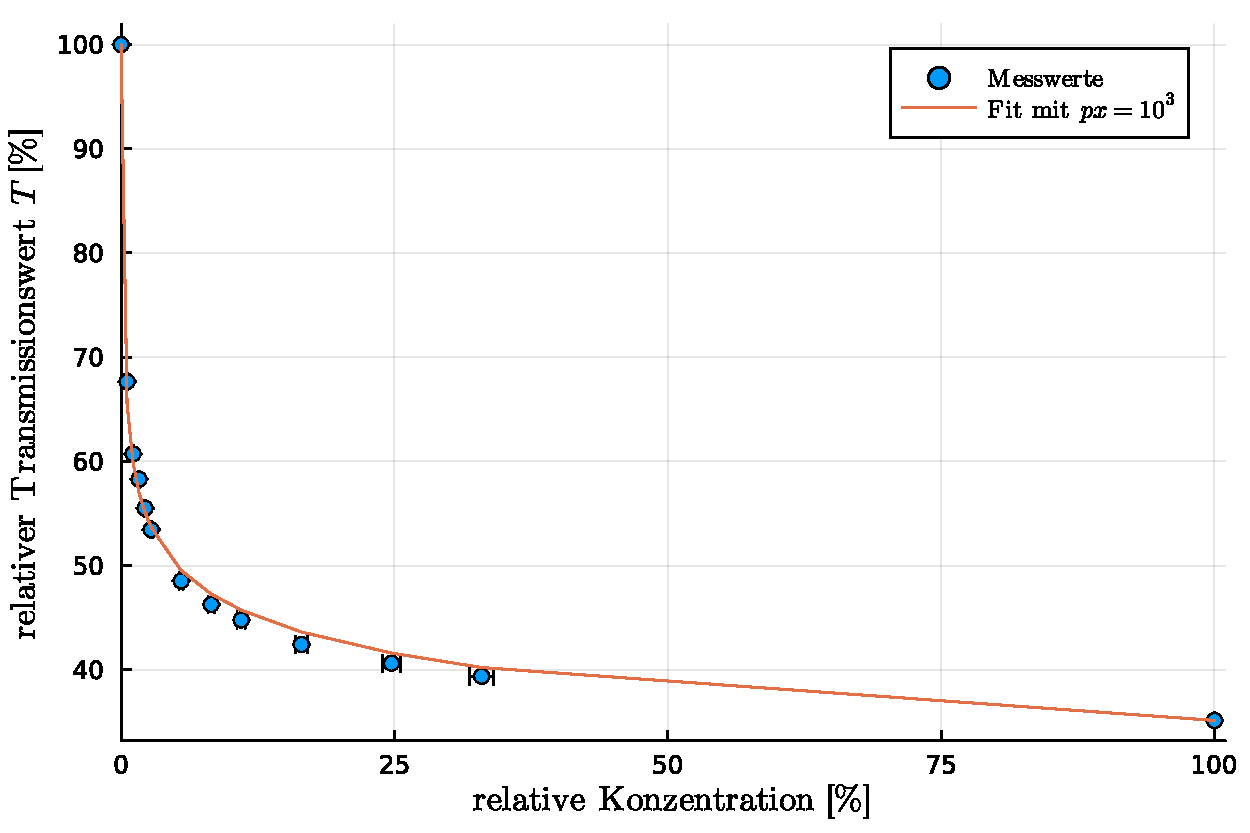
\includegraphics[width=0.7\textwidth]{../media/B1.1/tkFit.pdf}
	\caption{Gemessene Transmissionswerte verschiedener $\ce{CO_2}$--Konzentrationen (blau) und zugehöriger Fit (orange)}
	\label{abb:tkFit}
\end{figure}


\noindent
Für einen passenden Fit müssen die $T_\mathrm{rel}(C)$ um einen Faktor $F$ gestaucht und um einen Offset $O$ verschoben werden. Der Offset $O$ entspricht dem gemessenen Transmissionswert bei $100\%$ $\ce{CO_2}$, der Faktor $F$ entspricht dem Absorptionswert im selben Zustand.

\begin{eqnarray}
	\tilde{T}_\mathrm{rel}(C) &=& F \cdot T_{rel}(C) + O \\
	O &=& T_{mess}(100\%) \\
	F &=& 1 - O
\end{eqnarray}

\noindent
Zuletzt wurde der Fit--Parameter $px$ so angepasst, dass die Kurve möglichst gut mit Messwerten übereinstimmt. Dies ist für $px = 10^3$ der Fall.

Aufgrund der Form der Fit--Kurve ist die Empfindlichkeit des Spektrometers für kleine Konzentrationen größer, da dort bereits minimale Konzentrationsänderungen zu sichtbaren Änderungen des Transmissionswertes führen.

\subsubsection{minimale Konzentration}
\label{minimale Konzentration}
Nun soll die minimale Konzentration $K_\mathrm{min}$ ermittelt werden, die sich mit einer Unsicherheit von maximal $10 \mathrm{\,\%}$ bestimmen lässt. Dazu wird zunächst die Genauigkeit $\Delta I_\mathrm{therm}$ abgeschätzt, mit der ein Mittelwert von $I_0$ nach einer typischen Messung trotz thermischen Rauschens noch ermittelbar ist.

Dazu wird die Ungenauigkeit für jede einzelne Messung aller $\ce{CO_2}$--Konzentrationen $\Delta I_{\mathrm{therm}, i}$ abgeschätzt und anschließend gemittelt. Die Ungenauigkeit jeder einzelnen Messung ist durch den Fehler der Mittelwerte von $I_0$ darstellbar, der vor und nach jeder Messung bestimmt wird. Alle Fehler werden gemittelt um die Ungenauigkeit $\Delta I_\mathrm{therm}$ zu erhalten.

\begin{eqnarray}
	\Delta I_{\mathrm{therm}, i} &=& \frac{I_{0, i, \mathrm{vorher}} - I_{0, i, \mathrm{nachher}}}{2} \\
	\Delta I_\mathrm{therm} &=& \frac{1}{n} \sum_{i = 1}^{n} \Delta I_{\mathrm{therm}, i}
\end{eqnarray}

\noindent
Damit die minimale Transmission $T_\mathrm{min}$ erreicht ist, muss die Unsicherheit einer Transmissionsmessung genau $10 \mathrm{\, \%}$ betragen. Dazu muss die Differenz des Mittelwerts der Messwerte ohne $\ce{CO_2}$ $\bar{I}_{0}$ und des minimalen Messwerts mit $\ce{CO_2}$ $I_\mathrm{min}$ kleiner als das zehnfache der oben abgeschätzten Genauigkeit betragen.

\begin{eqnarray}
	\bar{I}_0 &=& \sum_{i=1}^{n} I_{0, i} \\
	\bar{I}_0 - I_\mathrm{min} &=& 10 \cdot \Delta I_\mathrm{therm} \\
	\Leftrightarrow \qquad I_\mathrm{min} &=& \bar{I}_0 - 10 \cdot \Delta I_\mathrm{therm}
\end{eqnarray}

\noindent
Der minimale Transmissionswert $T_\mathrm{min}$, der einer Ungenauigkeit von $10 \mathrm{\, \%}$ genügt, ergibt sich also folgenermaßen.

\begin{eqnarray}
	T_\mathrm{min} &=& \frac{I_\mathrm{min}}{\bar{I}_0} \\
	T_\mathrm{min} &\approx& 0.94
\end{eqnarray}

\noindent
Die minimale Konzentration $K_{min}$ wird anschließend mittels der Fit--Geraden $\tilde{T}_\mathrm{rel}(C)$ aus dem minimalen Transmissionswert ermittelt. Hierfür wird der obere Berecih des Fits vergrößert in Abbildung \ref{abb:fitZoom} dargestellt. Es wird deutlich, dass die minimale Konzentration $K_\mathrm{min}$ zwischen $300 \mathrm{\, ppm}$ und $400 \mathrm{\, ppm}$ liegen muss. Dementsprechend wird der Mittelwert inklusive der Fehler gebildet.

\begin{eqnarray}
	K_\mathrm{min} &=&  \frac{300 \mathrm{\, ppm} + 400 \mathrm{\, ppm}}{2} \\
	\Delta K_\mathrm{min} &=& \left|\frac{300 \mathrm{\, ppm} - 400 \mathrm{\, ppm}}{2}\right| \\
	K_\mathrm{min} &=& (350 \pm 50) \mathrm{\, ppm}
\end{eqnarray}

\begin{figure}[h]
	\centering
	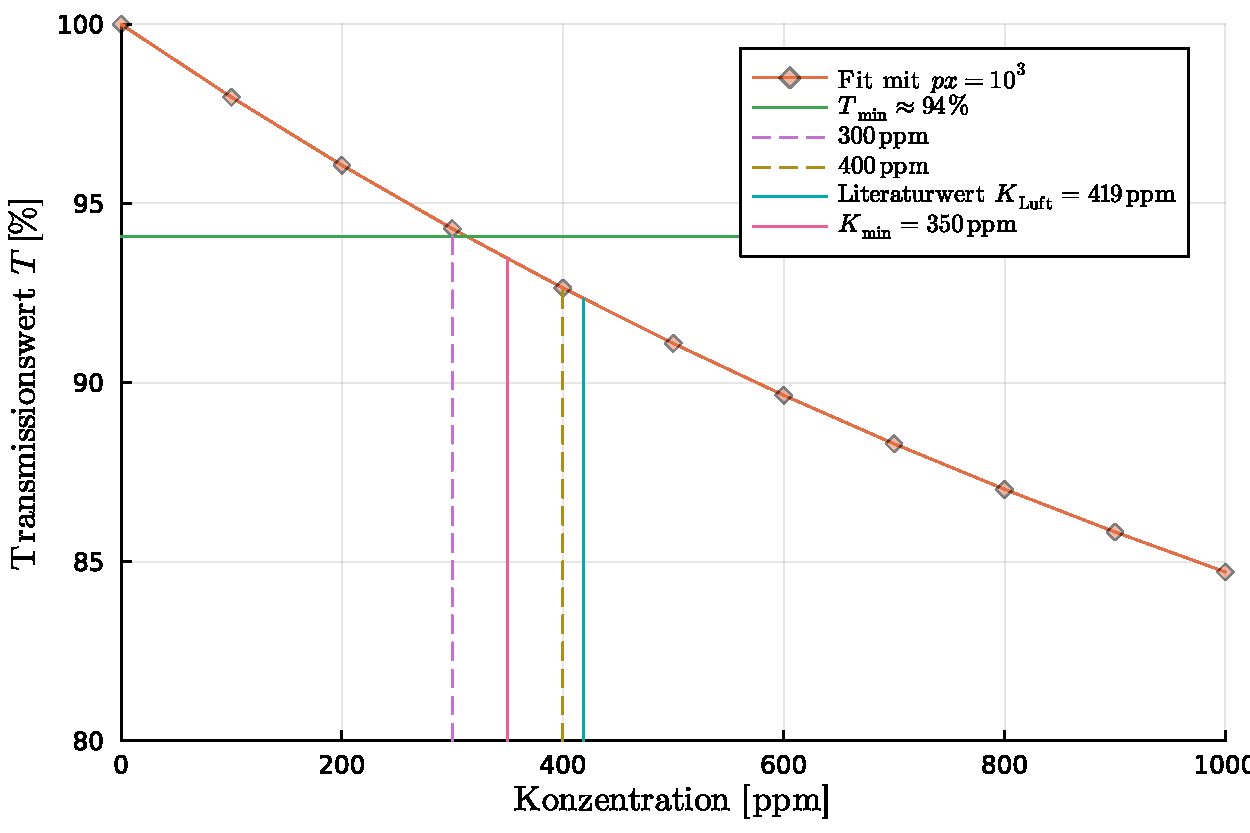
\includegraphics[width=0.7\textwidth]{../media/B1.1/fitZoomPpm.pdf}
	\caption{Darstellung der minimalen Konzentration $K_\mathrm{min}$,
		die noch mit einer Unsicherheit von $10 \mathrm{\, \%}$ bestimmt werden kann}
	\label{abb:fitZoom}
\end{figure}

\noindent
Der $\ce{CO_2}$--Gehalt in Luft beträgt laut Demtröder ca. $340 \mathrm{\, ppm}$ \cite{Demtröder Kern/Atom}.
Dies ist im Rahmen des Fehlers im Bereich der minimalen Konzentration $K_\mathrm{min}$. Daraus lässt sich folgern, dass der $\ce{CO_2}$--Gehalt der Luft sich mit diesem Spektrometer gut bestimmbar ist.

Das für diesen Versuchsteil verwendete Modell weist einige Annahmen auf, die vom realen Versuchsaufbau nicht bereitgestellt werden können. So wird beispielsweise die Glühwendel näherungsweise als schwarzer Körper betrachtet, was streng genommen nicht der Fall ist. Zudem sind beide zellabdeckenden Fenster nicht vollständig durchlässig für Infrarotstrahlung. Zuletzt befindet sich der Detektor außerhalb der Zelle, was zu einer zusätzlichen Abschwächung der Infrarotstrahlung durch Raumluft führt.

All diese Abweichungen führen dazu, dass das Lambert--Beer--Gesetz, aus dem sich die Lambert--Beer--Gauß--Funktion, und damit dieses Modell, ergibt, keine perfekte Beschreibung der Realität ermöglicht. Dennoch ist die Modellkurve sehr nah an den Messwerten. Dies zeigt, dass diese Abweichungen zwar einen bemerkbaren, aber keinen großen Einfluss auf das Ergebnis dieses Versuchsteils haben.

Der Temperaturabfall innerhalb der Zelle nach vollständigem Befüllen mit $\ce{CO_2}$ ist aller Wahrscheinlichkeit nach mit einer geringeren Temperatur innerhalb der Gasflasche als der des Stickstoffs zu erklären.

Nach vollständiger Befüllung der Zelle mit $\ce{CO_2}$ steigt die Temperatur in der Zelle langsam an und nähert sich dann einem konstanten Wert oberhalb der Starttemperatur. Bei erneuter Spülung mit Stickstoff nach der Messung sinkt die Temperatur zunächst wieder und steigt dann langsam auf den Wert vor der Messung.

Die erhöhte Temperatur während der Befüllung mit $\ce{CO_2}$ geht auf die infrarotaktiven Schwingungen der Gasmoleküle zurück, die eine Erhöhung der Temperatur hervorrufen.

\subsection{Spektrometrische Konzentrationsbestimmung}
\label{Spektrometrische Konzentrationsbestimmung}

Um die $\ce{CO_2}$--Konzentration der Raumluft zu bestimmen, wird zunächst die relative Transmission $T_\mathrm{rel, Luft}$ derselben berechnet.

\begin{figure}[h]
	\centering
	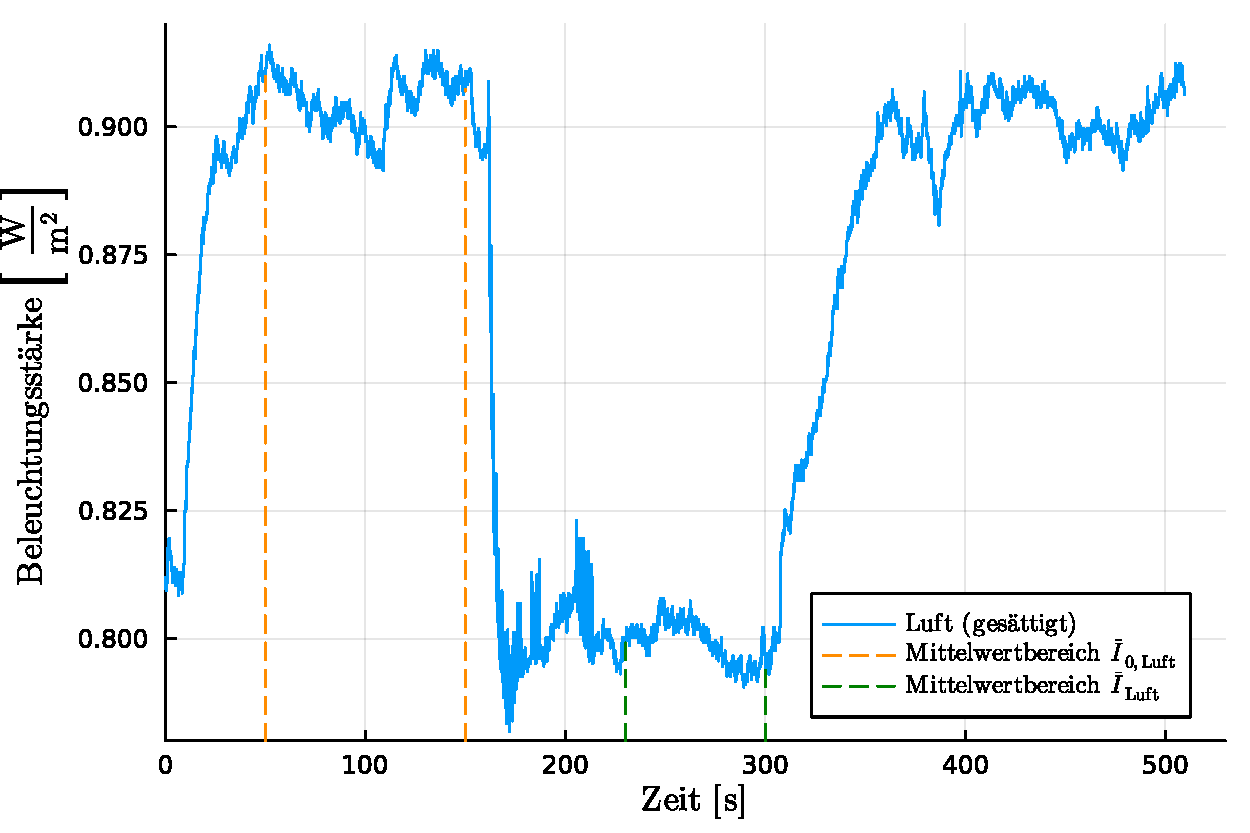
\includegraphics[width=0.7\textwidth]{../media/B1.1/luft.pdf}
	\caption{Gemessene Beleuchtungsstärke der Zelle gesättigt mit Raumluft (blau)\\
		und Bereiche für die Mittelwerte der Beleuchtungsstärken vor und nach einfüllen der Raumluft (gestrichelt)}
	\label{fig:luft}
\end{figure}

Dazu wir der Mittelwert der Beleuchtungsstärke vor und nach dem Befüllen mit Luft $\bar{I}_{0, \mathrm{Luft}}$ inklusive des jeweiligen Fehlers ermittelt. Die gemessene Beleuchtungsstärke der mit Raumluft gesättigten Zelle  sowie die für die jeweiligen Mittelwerte ausgesuchten Bereiche sind in Abbildung \ref{fig:luft} dargestellt.

Die relative Transmission der Luft $T_\mathrm{rel, Luft}$ berechnet sich aus dem Quotient beider Mittelwerte, der Fehler $\Delta T_\mathrm{rel, Luft}$ nach Gauß'scher Fehlerfortpflanzung.

\begin{eqnarray}
	\bar{I}_{0, \mathrm{Luft}} &=& (90.522\pm 0.017) \cdot 10^{-2} \mathrm{\,\frac{W}{m^2}}\\
	\bar{I}_\mathrm{Luft} &=& (79.949 \pm 0.015) \cdot 10^{-2} \mathrm{\, \frac{W}{m^2}} \\
	T_\mathrm{rel, Luft} &=& \frac{\bar{I}_\mathrm{Luft}}{\bar{I}_{0, \mathrm{Luft}}} \\
		&\approx& 88.320 \mathrm{\, \%} \\
	\Delta T_\mathrm{rel, Luft} &=&
		\sqrt{
			\left(
				\frac{\Delta \bar{I}_\mathrm{Luft}}{\bar{I}_{0, \mathrm{Luft}}}
			\right)^2
			+ \left(
				\frac{\bar{I}_\mathrm{Luft} \cdot \Delta \bar{I}_{0, \mathrm{Luft}}}{\bar{I}_{0, \mathrm{Luft}}^2}
			\right)^2
		} \\
	&\approx& 0.023 \mathrm{\, \%}
\end{eqnarray}

\noindent
Um nun die $\ce{CO_2}$--Konzentration der Raumluft zu bestimmen, wird erneut eine Fit--Gerade $\tilde{T}_\mathrm{rel}(C)$ verwendet. Hierfür wird wieder der obere Bereich vergrößert, was in Abbildung \ref{fig:luftZoom} zu sehen ist.

\begin{figure}[h!]
	\centering
	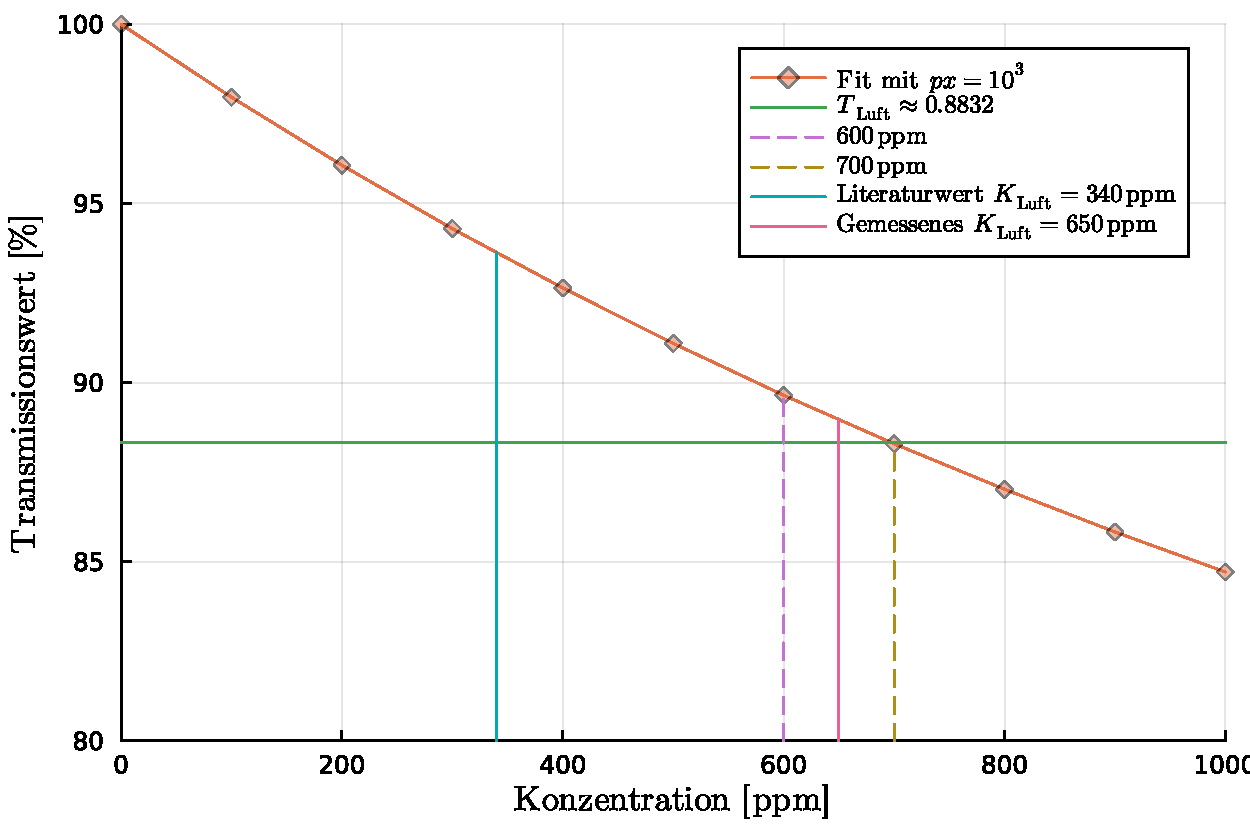
\includegraphics[width=0.7\textwidth]{../media/B1.1/luftZoomPpm.pdf}
	\caption{Darstellung der gemessenen $\ce{CO_2}$--Konzentration der Raumluft $K_\mathrm{Luft}$ anhand des oberen Endes des Fits der gemessenen Transmissionswerte verschiedener $\ce{CO_2}$--Konzentrationen}
	\label{fig:luftZoom}
\end{figure}

Es zeigt sich, dass  die zur oben bestimmten relativen Transmission gehörige $\ce{CO_2}$--Konzentration der Raumluft zwischen $600 \mathrm{\, ppm}$ und $700 \mathrm{\, ppm}$ liegen muss. Es wird also der Mittelwert inklusive Fehler gebildet und so die gemessene $\ce{CO_2}$--Konzentration der Raumluft $K_\mathrm{Luft}$ ermittelt.

\begin{eqnarray}
	K_\mathrm{Luft} &=& \frac{700 \mathrm{\, ppm} + 600 \mathrm{\, ppm}}{2} \\
	\Delta K_\mathrm{Luft} &=& \left|\frac{700 \mathrm{\, ppm} - 600 \mathrm{\, ppm}}{2}\right| \\
	K_\mathrm{Luft} = (650 \pm 50) \mathrm{\, ppm}
\end{eqnarray}

Dieser Wert entspricht auch innerhalb der Fehler nicht dem Literaturwert von $340 \mathrm{\, ppm}$ \cite{Demtröder Kern/Atom}. Dennoch ist er zumindest größenordnungsmäßig nah dran.

Die Abweichung lässt sich unter anderem damit erklären, dass sich während des gesamten Versuches mehrere Leute im Raum aufgehalten haben, was die $\ce{CO_2}$--Konzentration erhöht haben dürfte. Das Lüften des Raumes könnte nicht ausgereicht haben, um die $\ce{CO_2}$--Konzentration auf die Konzentration an der frischen Luft zu reduzieren.

\subsection{Drifteffekte}
\label{Drifteffekte}

Die Messkurve zeigt zu Beginn einen exponentiell abklingenden Anstieg, danach steigt die Kurve abschnittweise linear an. Hierfür sind die Drifteffekte verantwortlich, die eliminiert werden müssen. Das Rauschen, besonders der Peak am Anfang, entsteht wahrscheinlich durch einen Luftzug und durch Bewegungen im Raum.

Die Ursache für den Drift sind thermische Instabilitäten. Die IR--Quelle braucht eine gewisse Zeit, um ins Gleichgewicht zu kommen, in der Zwischenzeit können verschiedene Temperatureffekte auftreten. Zum einen erwärmt sich nicht nur die Glühwendel, sondern auch die umgebenden Materialien, sodass die Temperatur leicht ansteigt. Wenn die Temperatur der IR--Quelle sich ändert, gibt der IR--Detektor veränderte Signale aus. Temperaturempfindliche Bauteile wie z.B. der Verstärker oder elektrische Widerstände können ebenfalls einen Teil zum Intensitätsdrift beitragen.

Um die Driftanteile zu eliminieren, wird der Zeitpunkt $t_0\approx310\mathrm{\,s}$ benötigt, ab dem die Kurve konstant bleibt. Im Zeitintervall $[95\mathrm{\,s}, 310\mathrm{\,s}]$ kann man drei lineare Anstiege erkennen. Daher wird dieses Intervall in drei Teilintervalle $I_i$ aufgeteilt.

\begin{eqnarray}
	\begin{split}
		I_3 &=& [96,110] \\
		I_2 &=& [110,200] \\
		I_1 &=& [200,310]
	\end{split}
\end{eqnarray}

\noindent
Für jedes der Teilintervalle $I_i$ wird eine Geradengleichung $g_i(t)$ bestimmt.

\begin{eqnarray}
	g_1(t) &=&
	\begin{cases}
		1.179 \cdot 10^{-4} \mathrm{\,\frac{W}{s\cdot m^2}\,} \cdot t &: 0\mathrm{\,s\,}\leq t \leq 310 \mathrm{\,s\,} \\
		0.0365 \mathrm{\,\frac{W}{m^2}} &: t > 310
	\end{cases} \\
	g_2(t) &=&
	\begin{cases}
		1.883 \cdot 10^{-4} \mathrm{\,\frac{W}{s\cdot m^2}\,} \cdot t &: 0\mathrm{\,s\,}\leq t \leq 200 \mathrm{\,s\,} \\
		0.0377 \mathrm{\,\frac{W}{m^2}} &: t > 200
	\end{cases} \\
	g_3(t) &=&
	\begin{cases}
		7.058\cdot 10^{-4} \mathrm{\,\frac{W}{s\cdot m^2}\,} \cdot t &: 0\mathrm{\,s\,}\leq t \leq 110 \mathrm{\,s\,} \\
		0.0776 \mathrm{\,\frac{W}{m^2}} &: t > 110
	\end{cases}
\end{eqnarray}

\noindent
Zunächst wird die Gerade $g_1$ von der ursprünglichen Messkurve abgezogen. Dann wird die Steigung dieses Zwischenergebnisses ermittelt, woraufhin die Gerade $g_2$ bestimmt wird. Damit wird der Prozess wiederholt, ebenso für das letzte Intervall.

Zusätzlich wird von jedem Wert der dritten Kurve der Ordinatenwert $b=-0.014875224 \mathrm{\,\frac{W}{m^2}}$ subtrahiert, damit der Anstieg der Kurve bei $0\mathrm{\,\frac{W}{s\cdot m^2}}$ beginnt. Damit erhält man eine Messkurve ohne Driftanteile, die in Abbildung \ref{abb:Driftkorrektur der Messwerte} dargestellt ist.

Die Ergebnisse sind in Tabelle \ref{tab:rel Abweichung} dargestellt. Man sieht quantitativ, wie die ursprüngliche Kurve mit steigender Zeit immer mehr von der korrigierten Kurve abweicht.

\begin{figure}[h!]
	\centering
	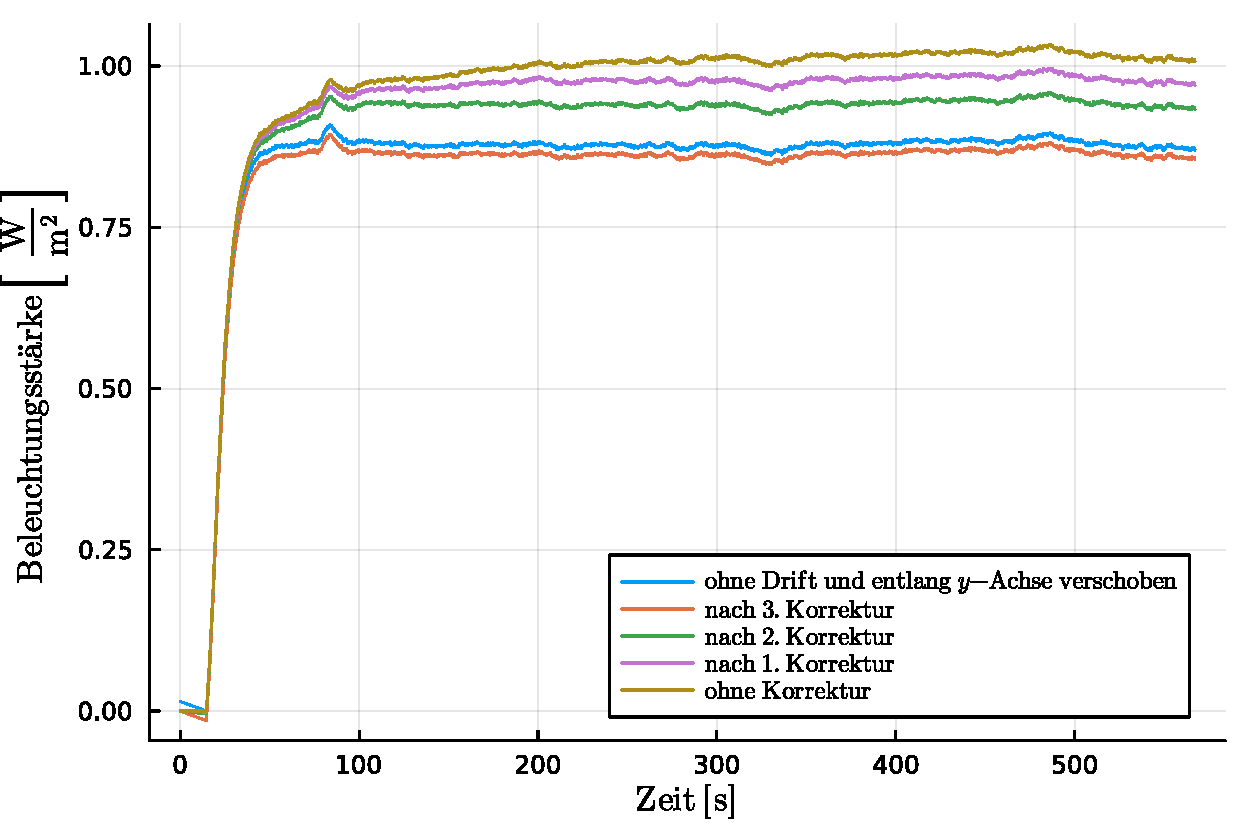
\includegraphics[width=0.7\textwidth]{../media/B1.1/Drift.pdf}
	\caption{Driftkorrektur der Messwerte}
	\label{abb:Driftkorrektur der Messwerte}
\end{figure}

\begin{table}[h!]
	\centering
	\begin{tabular}{c|c|c|c|c}
		Zeit $[\mathrm{s}]$
		& $I_\mathrm{D}$ $[\mathrm{\frac{W}{m^2}}]$
		& $I_\mathrm{oD}$ $[\mathrm{\frac{W}{m^2}}]$
		& Abweichung $[\mathrm{\frac{W}{m^2}}]$
		& relative Abweichung $[\%]$ \\
		\hline
		$100$ & $0.9696$ & $0.8838$ & $0.0858$ & $9.7\%$\\
		$200$ & $1.0039$ & $0.8801$ & $0.1201$ & $13.6\%$\\
		$300$ & $1.0125$ & $0.8768$ & $0.1287$ & $14.7\%$\\
	\end{tabular}
	\caption{Zunahme der relativen Abweichung zwischen der Beleuchtungsstärke ohne Drift $I_\mathrm{oD}$ und der mit Drift $I_\mathrm{D}$}
	\label{tab:rel Abweichung}
\end{table}

Nun soll noch ermittelt werden, ab welchem Zeitpunkt Messgenauigkeit mindestens $97\,\%$ beträgt. Dazu wird der Mittelwert von jeweils $100$ Messwerten zu verschiedenen Zeitpunkten gebildet und durch den Mittelwert von Messungen nach $310\mathrm{\,s}$ geteilt. Es stellt sich heraus, dass die relative Abweichung ab $t \approx 155.5\mathrm{\,s}$ kleiner als $3\%$ ist. Ohne Driftkorrektur ist eine Genauigkeit von $\geq 97\%$ schon nach ca. $53\mathrm{\,s}$ erreicht.

\subsection{Zeitkonstante}
\label{Zeitkonstante}
Nun soll die Zeitkonstante des Anschaltvorgangs $\tau$ durch einen Fit ermittelt werden.

Die driftkorrigierte Kurve wird mit $f(t)$ gefittet. $c$ ist der Wert, den die Funktion asymptotisch für $t \rightarrow \infty$ annähert, und wird durch den Mittelwert des stationären Bereiches dargestellt. $\tau $ ist die Zeitkonstante, die die Geschwindigkeit der Annäherung bestimmt. Da die Funktion bei $t=0\mathrm{\,s}$ beginnt, muss die Kurve auf der Zeitachse um $14.8\mathrm{\,s}$ verschoben werden.

\begin{eqnarray}
	f(t) &=& c \cdot \left(
	1 - \exp[-\frac{t}{\tau}]
	\right)
	\label{eq:Drift Fit} \\
	c &=& 0.8797 \mathrm{\,\frac{W}{m^2}}
\end{eqnarray}

\noindent
Zum Fitten wird das \code{Julia}--Paket \code{LsqFit} \cite{Julia:LsqFit} verwendet. Damit ergibt sich eine Zeitkonstante von ca. $23.7\mathrm{\,s}$. Der Fit ist in Abbildung \ref{abb:Fit für verschiedene tau} dargestellt.

\begin{eqnarray}
	\tau &=& (23.71 \pm 0.24)\mathrm{\,s}
\end{eqnarray}

\begin{figure}[h!]
	\centering
	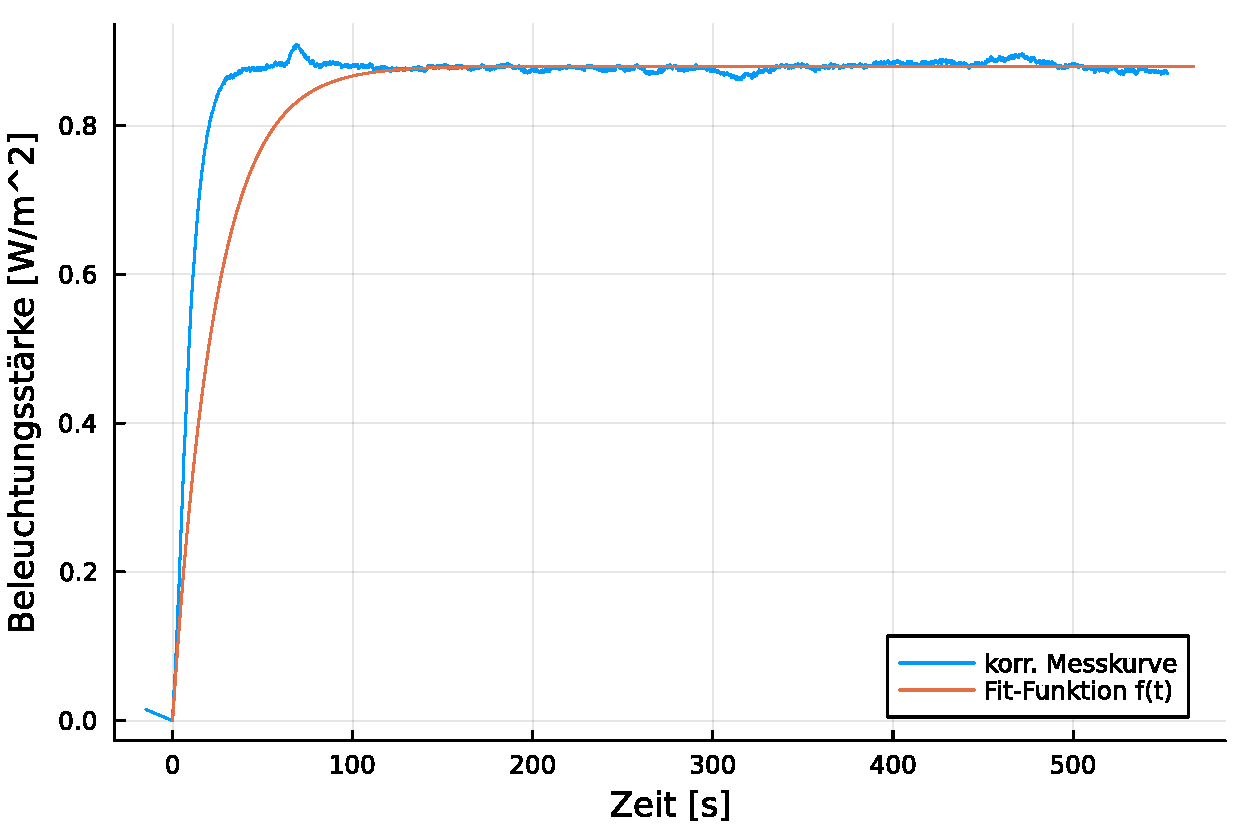
\includegraphics[width=0.7\textwidth]{../media/B1.1/ZeitkonstJulia.pdf}
	\caption{Gefittete Messkurve}
	\label{abb:Gefittete Messkurve}
\end{figure}

\noindent
Die gefittete Kurve steigt im Vergleich zu den Messdaten zu langsam an, auch wenn der stationäre Zustand sich bereits nach ca. $120\mathrm{\,s}$ eingestellt hat. Erst im stationären Zustand ist eine Beschreibung durch den Fit sinnvoll.

Zudem wurde manuell verschiedene Werte für $\tau$ ausprobiert. Hier fällt auf, dass der Anstieg nie richtig übereinstimmt. Entweder ist er zu langsam wie in Abbildung \ref{abb:Gefittete Messkurve} oder ist zu Beginn zu schnell und dann wieder zu langsam. Dieses Verhalten ist in Abbildung \ref{abb:Fit für verschiedene tau} zu sehen.

\begin{figure}[h!]
	\centering
	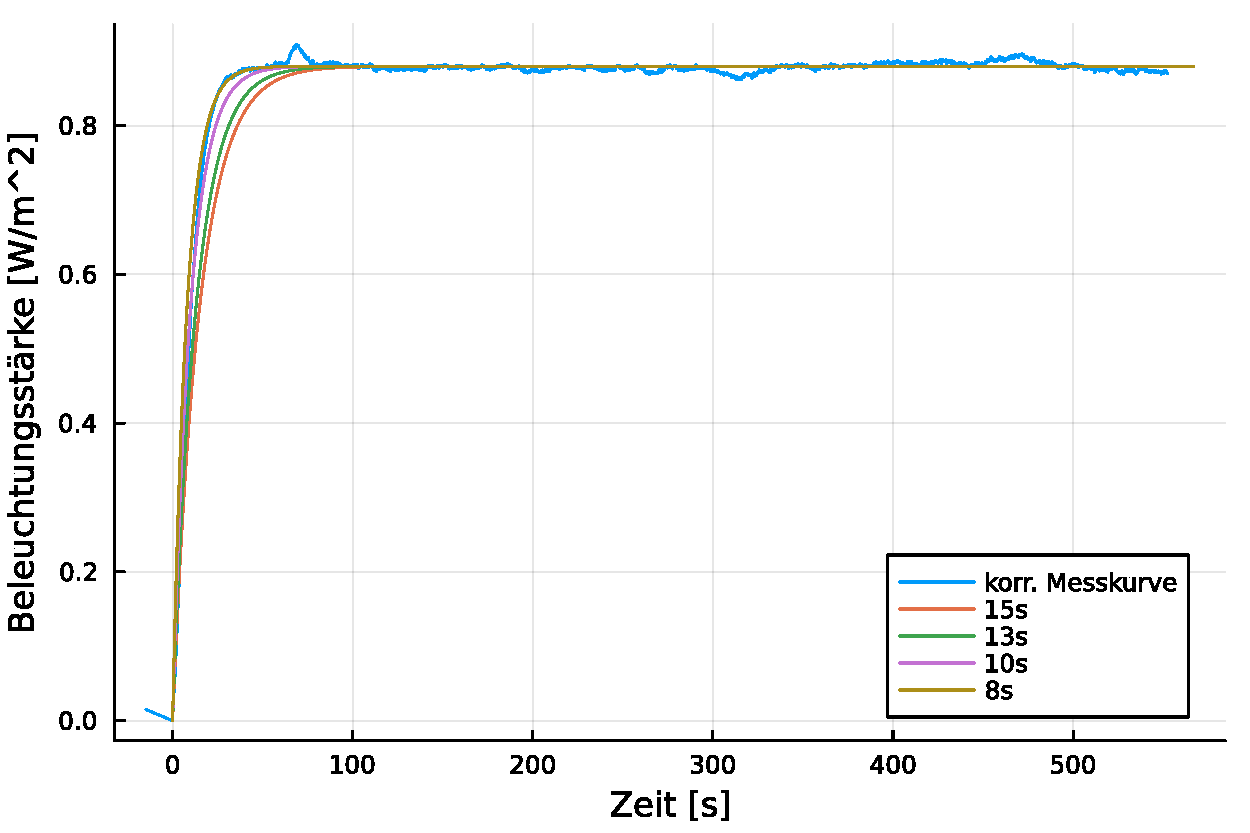
\includegraphics[width=0.7\textwidth]{../media/B1.1/versZeitkonst.pdf}
	\caption{Fit--Kurve für verschiedene $\tau$}
	\label{abb:Fit für verschiedene tau}
\end{figure}

\subsection{Optische Emission}
\label{Optische Emission}
Für alle Beteiligten war das Licht der Glühwendel bei einem Strom von $I\ge I_0=(7.1 \pm 0.1)\mathrm{\,A}$ zu sehen und bei $I\le (7.0 \pm 0.1)\mathrm{\,A}$ nicht mehr sichtbar. Daraus kann die Temperatur der Wendel ermittelt werden.

Für die Höchsttemperatur $T$ der Wendel gilt die folgende Näherung.

\begin{eqnarray}
	T &=& 79 \mathrm{\,\frac{K}{A}\,} \cdot I + 202\mathrm{\,K} \\
	\Delta T &=& 79 \frac{K}{A} \cdot \Delta I
\end{eqnarray}

\noindent
Daraus kann die Temperatur der Wendel $T(I_0)$ ermittelt werden. Weiterhin kann die Temperatur der Wendel bei maximalen Stromstärke $I_\mathrm{max} = (8.3 \pm 0.1)\mathrm{\,A}$ bestimmt werden.

%\begin{eqnarray}
%	T(I_0) &=& 762.9\mathrm{\,K} \pm 7.9\mathrm{\,K} \\
%	T(I_\mathrm{max}) &=& 857.71\mathrm{\,K} \pm 7.91\mathrm{\,K}
%\end{eqnarray}

%\noindent
Aus der Höchsttemperatur $T(I_\mathrm{max})$ kann die Wellenlänge $\hat \lambda$ mit der maximalen Strahlungsintensität über das Wien'sche Verschiebungsgesetz \eqref{eq:WienLambda} ermittelt werden. Der Fehler wird durch Gauß'sche Fehlerfortpflanzung bestimmt.

\begin{eqnarray}
	% \lambda(762.9\mathrm{\,K}) &\approx & 3.799 \cdot 10^{-6}\mathrm{\,m} \pm 3.934 \cdot 10^{-8}\mathrm{\,m} \\
	% \lambda(857.7\mathrm{\,K}) &\approx & 3.379 \cdot 10^{-6}\mathrm{\,m} \pm 3.934 \cdot 10^{-8}\mathrm{\,m} \\
	\Delta \hat  \lambda &= & 2.898 \cdot \mathrm{\,mm\,K\,}\cdot \frac{\Delta T}{{T}}
\end{eqnarray}

\noindent
Die Ergebnisse werden in Tabelle \ref{tab:Höchsttemperatur} zusammengefasst. Man sieht, dass die abgestrahlte Wellenlänge bei beiden Stromstärken im mittleren Infrarot--Bereich liegt.\footnote{Vergleiche Abschnitt \ref{elektromagnetisches-spektrum}}

\begin{table}[h!]
	\centering
	\begin{tabular}{c|c|c}
		Stromstärke $[\mathrm{A}]$ & $T(I)$ $[\mathrm{K}]$ & $\hat \lambda(T)$ $[\mathrm{\mu m}]$ \\
		\hline
		$7.1 \pm 0.1$ & $763 \pm 8$ & $ 3.80 \pm 0.04$  \\
		$8.3 \pm 0.1$ & $858 \pm 8$ & $ 3.38 \pm 0.04$  \\
	\end{tabular}
	\caption{Temperatur der Glühwendel $T(I)$ die mit höchster Intensität abgestrahlte Wellenlänge $\hat\lambda(T)$ bei verschiedenen Stromstärken}
	\label{tab:Höchsttemperatur}
\end{table}

\clearpage
\hypertarget{fazit}{%
\section{Fazit}\label{fazit}}

\clearpage
\hypertarget{literatur}{%
\section{Literatur}\label{literatur}}
\renewcommand{\section}[2]{} % remove extra title
\begin{thebibliography}{9}
\bibitem{UzK}
	Universität zu Köln, ``B1.1: Infrarotabsorption in $\ce{CO_2}$'', April 2024
\bibitem{BakanRaschke}
	S. Bakan \& E. Raschke, ``Der natürliche Treibhauseffekt'', Promet 28,
	Deutscher Wetterdienst, 2002, Online verfügbar unter
	\url{https://www.dwd.de/DE/leistungen/pbfb_verlag_promet/pdf_promethefte/28_3_4_pdf.pdf}
\bibitem{Demtröder Atom}
	W. Demtröder, ``Experimentalphysik 3: Atome, Moleküle und Festkörper'',
	Springer--Spektrum--Verlag, 5. Auflage 2016,
	DOI~\href{https://doi.org/10.1007/978-3-662-49094-5}{10.1007/978-3-662-49094-5}
\bibitem{Demtröder Kern/Atom}
	W. Demtröder, ``Experimentalphysik 4: Kern-, Teilchen- und Astrophysik'',
	Springer--Spektrum--Verlag, 5. Auflage 2017, DOI~\href{https://doi.org/10.1007/978-3-662-52884-6}{10.1007/978-3-662-52884-6}
\bibitem{Gerthsen}
	D. Meschede, ``Gerthsen Physik'', 21. Auflage, Springer Verlag,
	DOI~\href{https://doi.org/10.1007/978-3-662-45977-5}{10.1007/978-3-662-45977-5}
\bibitem{HakenWolf}
	H. Haken \& H. Wolf, ``Molekülphysik und Quantenchemie'', Springer-Verlag, 2006,
	DOI~\href{https://doi.org/10.1007/3-540-30315-4}{10.1007/3-540-30315-4}
\bibitem{Strahldichte}
	Wikipedia, ``Strahldichte'',
	\url{https://de.wikipedia.org/wiki/Strahldichte}, Abruf am 02.05.2024
\bibitem{abb:SpektrumSK}
	Wikipedia, \url{https://commons.wikimedia.org/wiki/File:BlackbodySpectrum_lin_150dpi_de.png},
	Abruf am 02.05.2024
\bibitem{Dipolmoment}
	Lexikon der Physik, ``Dipolmoment'',
	\url{https://www.spektrum.de/lexikon/physik/elektrisches-dipolmoment/3960},
	Abruf am 02.05.2024
\bibitem{Hinderer}
	F. Hinderer, ``UV/Vis--Absorptions- und Fluoreszenz--Spektroskopie'',
	2020,
	DOI~\href{https://doi.org/10.1007/978-3-658-25441-4}{10.1007/978-3-658-25441-4}
\bibitem{Fließbach}
	T. Fließbach, ``Statistische Physik'', 2018,
	DOI~\href{https://doi.org/10.1007/978-3-662-58033-2}{10.1007/978-3-662-58033-2}
\bibitem{Freiheitsgrad}
	Technische Falkutät Kiel, ``Freiheitsgrade der Rotation'',
	\url{https://www.tf.uni-kiel.de/matwis/amat/mw1_ge/kap_5/advanced/t5_2_4.html},
	Abruf am 03.05.2024
\bibitem{abb:gaussians}
	Wikimedia,
	\url{https://commons.wikimedia.org/wiki/File:Normal_Distribution_PDF.svg},
	2023-02-23
\bibitem{GoodyYung}
	R. M. Goody \& Y. L. Yung, ``Atmospheric Radiation: Theoretical Basis'', 1995,
	DOI  (der 2. Auflage) \href{https://doi.org/10.1093/oso/9780195051346.001.0001}{10.1093/oso/9780195051346.001.0001}
\bibitem{Einsiedler}
	M. Einsiedler, ``Analysis I: Kapitel $1$-$9$'', 2022,
	\url{https://wp-prd.let.ethz.ch/analysis19/chapter/treppenfunktionen-und-deren-integral},
	Abruf am 03.05.2024
\bibitem{abb:Schwingungen CO2}
	Wikimedia, ``File:Co2 vibrations.svg''
	\url{https://commons.wikimedia.org/wiki/File:Co2_vibrations.svg}
\bibitem{pyroelektrischer Sensor}
	Michael Muth, ``Pyrosensoren'', 1998,
	\url{https://www.michael-muth.de/lectures/TempSens/chap06.html}, Abruf am 12.06.2024
\bibitem{Wikipedia: Elektromagnetisches Spektrum}
	Wikimedia, ``File:Electromagnetic spectrum -de c.svg'',
	\url{https://commons.wikimedia.org/wiki/File:Electromagnetic_spectrum_-de_c.svg}, Abruf am 12.06.2024
\bibitem{Agilent Technologies}
	Agilent Technologies, ``Die Grundlagen der Spektroskopie'', 2016
	\url{https://www.agilent.com/Library/eseminars/Public/5991-6594_Agilent_Spectroscopy_Theory_DEE.pdf},
	Abruf am 10.06.2024
\bibitem{Julia:LsqFit}
	\code{\href{https://julialang.org}{Julia}}--Paket \code{LsqFit},
	Dokumentation unter \url{https://docs.juliahub.com/General/LsqFit/stable}
\end{thebibliography}
\end{document}
